\documentclass{article}
\usepackage{geometry}
\geometry{hmargin=2.5cm}
\usepackage{enumitem}
\setlist[enumerate]{label*=\arabic*.}
\usepackage{fancyhdr}
\usepackage{amsmath}
\usepackage{graphicx}
\usepackage{subcaption}
\usepackage{float}
\usepackage{hyperref}
\usepackage{gensymb}
\usepackage{siunitx}
\usepackage{wasysym}


\title{Capteurs \\
    \large Dossier reprenant les exercices réalisés au cours}
\date{2019 - 2020}
\author{Laura Binacchi}

\begin{document}
\pagenumbering{gobble}
\maketitle
\newpage
\tableofcontents
\newpage
\pagenumbering{arabic}
\pagestyle{fancy} 
\lhead{Laura Binacchi}
\rhead{Capteurs 2019-2020}

\section{Précision : PT 100 (16 décembre 2019)}
\paragraph{Énoncé}
Ce capteur mesure une température de 100\degree C. Quelle est l'erreur maximum commise sur cette température ?

\begin{figure}[H]
    \centering
    \begin{subfigure}[b]{0.4\linewidth}
        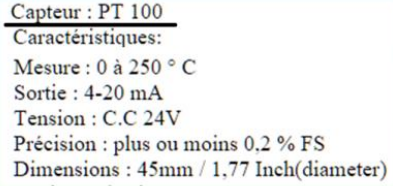
\includegraphics[width=\linewidth]{./images/002-precision-pt-100.png}
    \end{subfigure}
    \begin{subfigure}[b]{0.2\linewidth}
        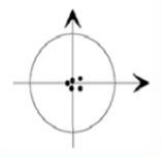
\includegraphics[width=\linewidth]{./images/003-precision-pt-100.png}
    \end{subfigure}
\end{figure}

\paragraph{Réponse}
Ce capteur va de 0 à 250\degree C. L'étendue de mesure est donc de 250\degree C. La précision étant de de $\pm 0.2\%$, l'erreur maximum est de $\pm 0.2\% \times 250\degree C = \pm 0.5\degree C$. La température mesurée de 100\degree C est donc en réalité comprise entre \SI{99.5}{\celsius} et \SI{100.5}{\celsius}.

\section{Linéarité : PT 100 et thermistance (16 décembre 2019)}
\paragraph{Énoncé}
Ces capteur sont-ils linéaires ?
\begin{itemize}
    \item PT 100 : $R_{\left(T\right)} = R0\left(1 + aT\right)$
    \item Thermistance : $R_{\left(T\right)} = a.e^{\frac{b}{T}}$
\end{itemize}

\paragraph{Réponse}
La PT 100 est linéaire (équation linéaire) mais la thermistance ne l'est pas.


\newpage
\section{Déterminer de la sensibilité d'un circuit (16 décembre 2019)}
\paragraph{Énoncé}
On désire acquérir la température ambiante d'une salle. Pour cela, on utilise un capteur de température qui est une sonde PT 100 possédant une résistance $R_{\theta}$ qui dépend de la température $\theta$ suivant la relation $R_\theta = R_0\left(1 + a\theta \right)$ avec :
\begin{itemize}
    \item[] $R_0 = \SI{100}{\ohm}$ ; $a = 0,4\degree C^{-1}$ ; $\theta$ = température en \degree C
\end{itemize}

Le monteur conditionneur suivant permet de traduire la température $\theta$ en une tension. On donne $R_2 = R_3 = \SI{1}{\kilo\ohm}$, $R_1 = \SI{3}{\kilo\ohm}$ et $V_{cc} = \SI{12}{\volt}$.

\begin{figure}[H]
    \centering
    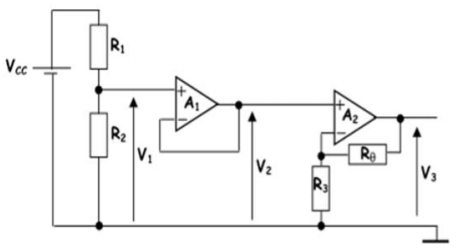
\includegraphics[width=0.6\linewidth]{./images/003-ex-sensibilite.png}
\end{figure}

\begin{enumerate}
    \item Montrer que la tension $V_3$ s'écrit $V_3 = (0,12\theta) + 3,3$.
    \item Calculer la sensibilité du montage définie par : $S_m = \frac{\partial V_3}{\partial\theta}$.
    \item Tracer et relever la caractéristique $V_\theta$ sous le simulateur Qucs.
\end{enumerate}

\subsection{Déterminer V3}
\paragraph{}
Montrer que la tension $V_3$ s'écrit $V_3 = (0,12\theta) + 3,3$.

\paragraph{}
Déterminer $V_1$ :
\begin{align*}
    V_1 & = \frac{V_{cc} . R_2}{R_1 + R_2}  \\
    V_1 & = \frac{12 . 10^3}{3.10^3 + 10^3} \\
    V_1 & = \SI{3}{\volt}
\end{align*}

\paragraph{}
Déterminer $V_2$ :
\begin{equation*}
    V_2 = V_1 = \SI{3}{\volt}
\end{equation*}
\paragraph{}
Car $A_1$ est monté en buffer.

\subparagraph{}
Déterminer $V_3$ :
$A_2$ est monté en non inverseur et on a $R_\theta = R_0\left(1 + a\theta \right)$ et $a = 0,4\degree C^{-1}$.
\begin{align*}
    V_3 & = V_2\left(1 + \frac{R_\theta}{R_3}\right)                      \\
    V_3 & = V_2\left(1 + \frac{R_0\left(1 + a\theta \right)}{R_3}\right)  \\
    V_3 & = 3\left(1 + \frac{100\left(1 + 0,4\theta \right)}{10^3}\right) \\
    V_3 & = \frac{3.10^3 + 300 + 120\theta}{10^3}                         \\
    V_3 & = 3,3 + 0,12\theta
\end{align*}

\subsection{Calculer la sensibilité du montage}
\paragraph{}
définie par : $S_m = \frac{\partial V_3}{\partial\theta}$ : $$S_m = 0,12 = 120 \si{\milli\volt/\celsius}$$

\paragraph{}
La sensibilité étant constante, on peut en déduire que le capteur est linéaire.

\subsection{Qucs}
\paragraph{}
Tracer et relever la caractéristique $V_\theta$ sous le simulateur Qucs.

\paragraph{Déterminer la plage de fonctionnement de la PT 100 :}

\paragraph{}
Température maximale :
\begin{align*}
    V_{3 max}    & = 15 = 3,3 + 0,12\theta_{max} \\
    \theta_{max} & = \frac{15 - 3,3}{0,12}       \\
    \theta_{max} & = 97,5\si{\celsius}
\end{align*}

\paragraph{}
Résistance maximale :
\begin{align*}
    R_{\theta max} & = R_0\left(1 + a\theta_{max} \right) \\
    R_{\theta max} & = 100\left(1 + 0,4 . 97,5\right)     \\
    R_{\theta max} & = \SI{4000}{\ohm}
\end{align*}

\paragraph{}
La résistance interne de la PT 100 varie donc entre 100 et 4000\si{\ohm}.

\newpage
\paragraph{Réalisation sur Qucs}\
\begin{figure}[H]
    \centering
    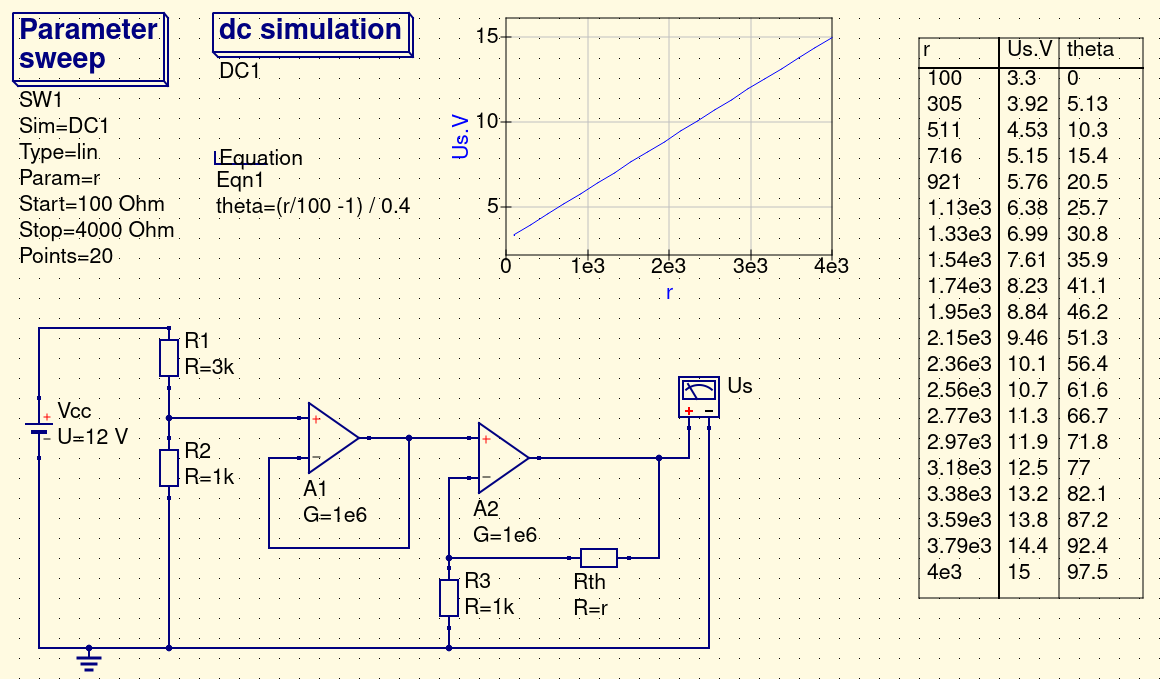
\includegraphics[width=\linewidth]{./images/003-qucs.png}
\end{figure}


\newpage
\section{Étalonnage d'un capteur avec un tableur (1) (16 décembre 2019)}

\paragraph{Reproduire l'exemple suivant : }
On prépare des solutions étalons et on mesure leur conductance à l'aide d'un conductimètre. Les valeurs de concentrations et de conductances de ces solutions sont reportées dans le tableau ci-dessous :

\begin{table}[H]
    \begin{center}
        \begin{tabular}{l|c|c|c|c|c|c}
            \textbf{c (\SI{}{\mol\per\liter})} & 1,00 & 0,70 & 0,49 & 0,21 & 0,10 & 0,00 \\
            \hline
            \textbf{G (\SI{}{\milli\siemens})} & 1,30 & 0,89 & 0,66 & 0,28 & 0,12 & 0,00 \\
        \end{tabular}
    \end{center}
\end{table}

\paragraph{}
On demande de/d'
\begin{itemize}
    \item tracer la courbe d'étalonnage correspondant à ces mesures sous Excel;
    \item afficher l'équation de la courbe correspondant au nuage de points obtenus et le coefficient de corrélation de la courbe.
\end{itemize}
NB. La concentration molaire du soluté est $c = \frac{n}{V}$ où n est la quantité de matière de soluté (mol) et V le volume de solution (L).

\paragraph{Réalisation}
\
\begin{figure}[H]
    \centering
    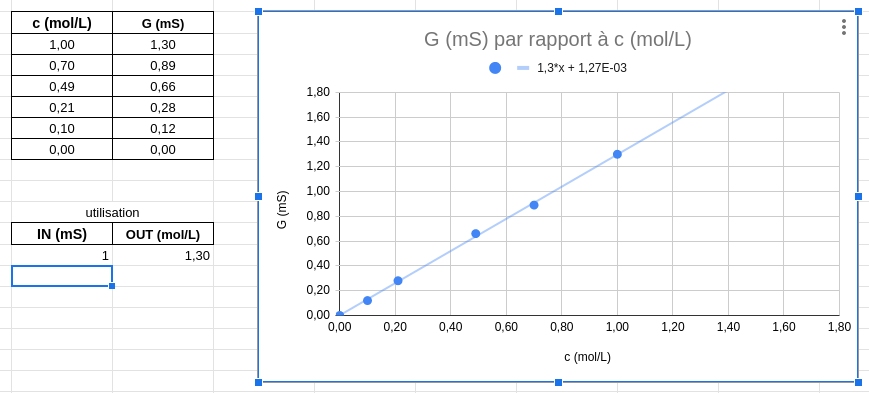
\includegraphics[width=\linewidth]{./images/004-etalonnage-exemple.png}
\end{figure}

\newpage
\section{Étalonnage d'un capteur avec un tableur (2) (16 décembre 2019)}

\paragraph{Énoncé}
On chauffe un ballon contenant de l'eau et de la glace jusqu'à ébullition. La thermistance est immergée dans ce milieu ainsi qu'un thermomètre pour suivre l'évolution de la température. La résistance est reliée à un ohmmètre.

\begin{table}[H]
    \centering
    \begin{tabular}{l|c|c|c|c|c|c|c|c|c|c}
        \textbf{Température (\SI{}{\celsius})} & 0    & 5    & 10   & 15   & 20   & 25   & 30   & 35   & 40   & 45   \\
        \hline
        \textbf{Résistance (\SI{}{\kilo\ohm})} & 6,40 & 4,78 & 4,06 & 3,26 & 2,53 & 2,03 & 1,63 & 1,31 & 1,05 & 0,85 \\
        \hline
        \textbf{Température (\SI{}{\celsius})} & 50   & 55   & 60   & 65   & 70   & 75   & 80   & 85   & 90   & 95   \\
        \hline
        \textbf{Résistance (\SI{}{\kilo\ohm})} & 0,69 & 0,56 & 0,46 & 0,38 & 0,32 & 0,28  & 0,22 & 0,19 & 0,16 & 0,14 \\
    \end{tabular}
\end{table}

\paragraph{}
On demande de tracer la courbe d'étalonnage du capteur sur le tableur Excel et de donner l'équation de la courbe de tendance.

\paragraph{Réalisation}
\
\begin{figure}[H]
    \centering
    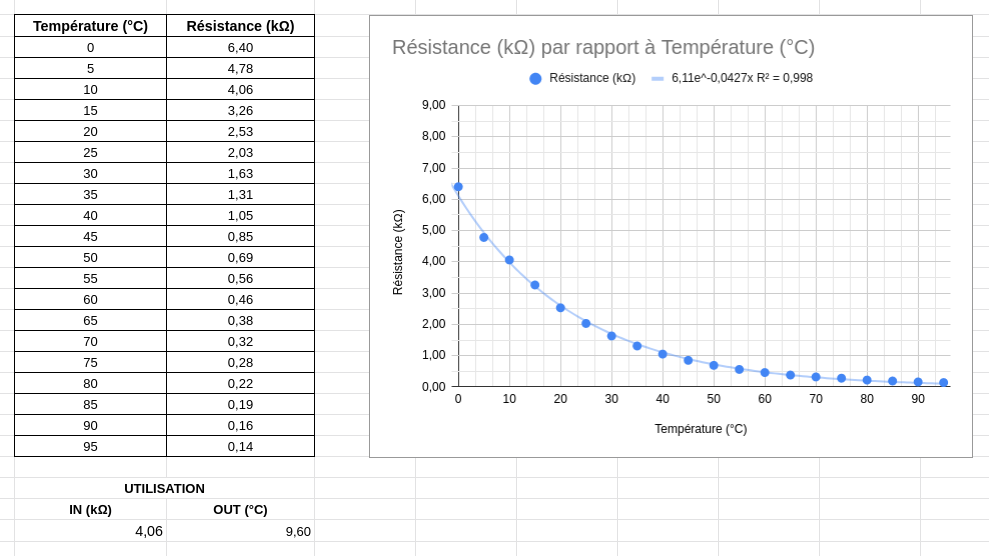
\includegraphics[width=\linewidth]{./images/005-etalonnage-exercice.png}
\end{figure}

\newpage
\section{Équation aux dimensions (6 janvier 2020)}
\subsection{Exemples}
\begin{itemize}
    \item L'équation aux dimensions de la force est
          \begin{equation*}
              F = MLT^{-2}
          \end{equation*}
          puisque $F = m.a$ et l'unité SI est le $\si{\kilogram \meter \per \square \second}$ ou Newton.
    \item Pour l'énergie, l'équation aux dimensions est
          \begin{equation*}
              W = ML^2T^{-2}
          \end{equation*}
          puisque $ W = \frac{1}{2}m.v^2$ et l'unité SI est le $\si{\kilogram \square \meter \per \square \second}$ ou Joule.
\end{itemize}

\subsection{Exercice}
La formule $E = mc^2$ est-elle homogène ?

\paragraph{Réponse}
La dimension de $E = ML^2T^{-2}$ puisque l'unité de E est le Joule ou $\si{\kilogram \square \meter \per \square \second}$. La dimension de $m.c^2 = M.\left(\frac{L}{T}\right)^2 = ML^2T^{-2}$. Les dimensions correspondent. L'équation est donc bien homogène.

\subsection{Dimension d'une grandeur dérivée}
\paragraph{Énoncé}
Analyse dimensionnelle des grandeurs dérivées suivantes :
\begin{itemize}
    \item La résistance électrique
    \item La fréquence
    \item La vitesse
    \item La force
    \item La pression
    \item Le débit volumique
    \item La charge électrique
    \item L'énergie
\end{itemize}

\newpage
\paragraph{Réponse}
\subparagraph{La fréquence}
La fréquence est exprimée en Hertz $= \SI{1}{\per \second}$. Sa dimension est : $$T^{-1}$$

\subparagraph{La vitesse}
La fréquence est exprimée en $= \si{\meter \per \second}$. Sa dimension est : $$LT^{-1}$$

\subparagraph{La force}
La force $F = m.a$ s'exprime en $\si{\kilogram \meter \per \square \second}$ (ou Newton). Sa dimension est : $$LMT^{-2}$$

\subparagraph{La pression}
La pression $P = \frac{F}{S}$ exprimée en $\si{\newton \per \square \meter}$ ou $\si{\kilogram \per \meter \per \square \second}$. Sa dimension est : $$L^{-1}MT^{-2}$$

\subparagraph{Le débit volumique}
Le débit volumique s'exprime en $\frac{V}{s}$ ou $\frac{m^3}{s}$. Sa dimension est : $$L^3T^{-1}$$

\subparagraph{La charge électrique}
$I = \frac{Q}{t} \Rightarrow Q = \frac{I}{t}$. La charge électrique Q s'exprime en $\si{\ampere \per \second}$. Sa dimension est : $$T^{-1}I$$

\subparagraph{L'énergie}
L'unité de E est le Joule ou $\si{\kilogram \square \meter \per \square \second}$. Sa dimension est : $$L^2MT^{-2}$$

\subparagraph{La résistance électrique}
La dimension de la résistance est déterminée par l'intermédiaire de celle de la puissance car $P = R.I^2 \Rightarrow R = \frac{P}{I^2}$.

La puissance $P = \frac{E}{t}$. Sa dimension est : $$L^2MT^{-3}$$

La dimension de R est donc : $$L^2MT^{-3}I^{-2}$$

\newpage
\section{Les grandeurs physiques (6 janvier 2020)}
\subsection{Le Kelvin}
\paragraph{Énoncé}
A combien de degrés Kelvin correspondent \SI{20}{\celsius} ?

\paragraph{Réponse}
$\SI{20}{\celsius} = \SI{293,15}{\kelvin}$

\subsection{La pression}
\paragraph{Énoncé}
Combien vaut \SI{1}{\milli \bar} en \si{\kilo \pascal} ? en \si{\hecto \pascal} ?

\paragraph{Réponse}
$\SI{1}{\milli \bar} = 0,1\si{\kilo \pascal} = \SI{1}{\hecto \pascal}
$

\subsection{Les longueurs d'ondes}
\paragraph{Énoncé}
Quelle est la fréquence en \si{\kilo\hertz} correspondant à une longueur d'onde de \SI{2000}{\meter} ?

\paragraph{Réponse}
$\lambda = \frac{c}{f} \Rightarrow f = \frac{c}{\lambda} = \frac{3.10^8}{2000} = \SI{150}{\kilo\hertz}$


\newpage
\section{Capteur de force (6 janvier 2020)}
\paragraph{Énoncé}
\paragraph{}
Un capteur de force est constitué de 4 jauges de contrainte collées sur une pièce métallique appelée corps d'épreuve. Les jauges de contrainte sont des conducteurs ohmiques dont la résistance varie sous l'effet de la déformation qui apparaît lorsque le corps d'épreuve est soumis à la force F que l'on désire mesurer.

\paragraph{}
Pour augmenter la sensibilité du dispositif, les jauges sont montées en pont, appelé pont de Wheatstone (montage ci-dessous). En l'absence de forces, les 4 résistances sont identiques, de valeur nominale $R_0$. En présence de forces, 2 jauges sont en extension et voient leur résistance augmenter : $r_1 = r_4 = R_0 + \Delta R$. Les deux autres, en compression, voient leur résistance diminuer : $r_2 = r_3 = R_0 - \Delta R$.

\paragraph{}
La variation $\Delta R$ vérifie la relation $\frac{\Delta R}{R_0} = k.F$

\begin{figure}[H]
    \centering
    \begin{subfigure}[b]{0.4\linewidth}
        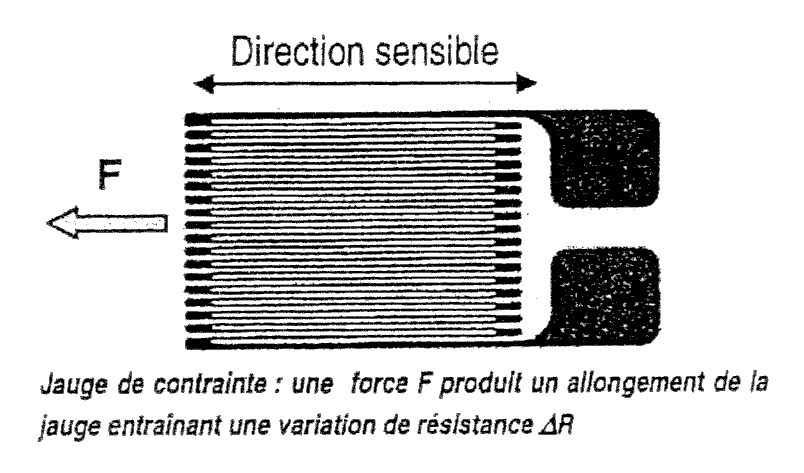
\includegraphics[width=\linewidth]{./images/capteur-force-1.png}
    \end{subfigure}
    \begin{subfigure}[b]{0.5\linewidth}
        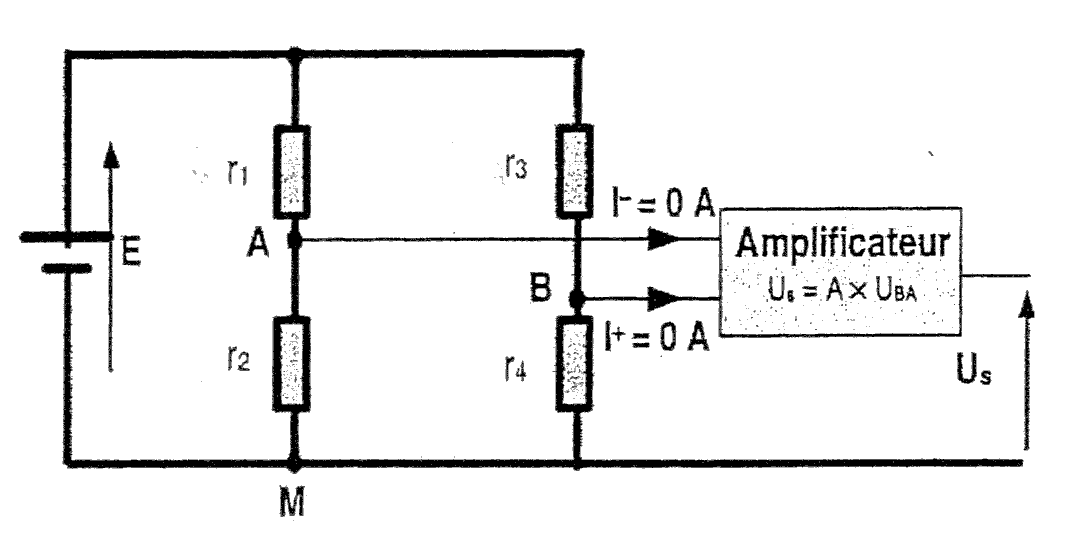
\includegraphics[width=\linewidth]{./images/capteur-force-2.png}
    \end{subfigure}
\end{figure}

\paragraph{}
\begin{enumerate}
    \item Exprimer $U_AM$ en fonction de E, $R_0$ et $\Delta R$.
    \item Exprimer $U_BM$ en fonction de E, $R_0$ et $\Delta R$.
    \item En déduire que $U_BA = \frac{\Delta R}{R_0} E$.
    \item Montrer que la tension $U_S$ est proportionnelle à la force F.
    \item Lorsque l'on soumet le corps d'épreuve à une Force $F_0 = \SI{1000}{\newton}$, on mesure $U_{S0} = \SI{440}{\milli\volt}$. Exprimer k puis calculer sa valeur numérique (on précisera également son unité). Calculer $\Delta R$.
\end{enumerate}

\paragraph{}
On donne : $E = \SI{10}{\volt}$, $A = 100$, $R_0 = \SI{350}{\ohm}$

\subsection{Expression de $U_{AM}$}
\begin{align*}
    U_{AM} & = \frac{E.R_2}{R_1 + R_2}\\
    U_{AM} & = \frac{E(R_0 - \Delta R)}{R_0 + \Delta R + R_0 - \Delta R }\\
    U_{AM} & = \frac{E(R_0 - \Delta R)}{2R_0}\\
\end{align*}

\subsection{Expression de $U_{BM}$}
\begin{align*}
    U_{BM} & = \frac{E.R_4}{R_3 + R_4}\\
    U_{BM} & = \frac{E(R_0 + \Delta R)}{2R_0}\\
\end{align*}

\subsection{Expression de $U_{BA}$}
\begin{align*}
    U_{BA} & = U_{BM} - U_{AM}\\
    U_{BA} & = \frac{E(R_0 + \Delta R)}{2R_0} - \frac{E(R_0 - \Delta R)}{2R_0}\\
    U_{BA} & = \frac{E.R_0 + E.\Delta R - E.R_0 + E.\Delta R}{2R_0}\\
    U_{BA} & = \frac{E.\Delta R}{R_0}\\
\end{align*}

\subsection{Montrer que le tension de sortie est proportionnelle à la force appliquée}

$$\frac{\Delta R}{R_0} = k.F \Rightarrow U_{BA} = E.k.F \Rightarrow U_S = A.E.k.F$$

\subsection{Calcul de k et $\Delta R$}
Avec $F_0 = \SI{1000}{\newton}$, $U_{S0} = \SI{440}{\milli\volt}$, $E = \SI{10}{\volt}$, $A = 100$ et $R_0 = \SI{350}{\ohm}$
\paragraph{}
$$ k = \frac{U_{S0}}{A.E.F_0} = \frac{440.10^{-3}}{100.10.1000} = 440.10^{-9} \si{\per\newton}$$

$$\Delta R = R_0.k.F_0 = 350.440.10^{-9}.1000 = \SI{154}{\milli\ohm}$$


\newpage
\section{Conditionneur d'une balance (6 et 13 janvier)}
\begin{figure}[H]
    \centering
    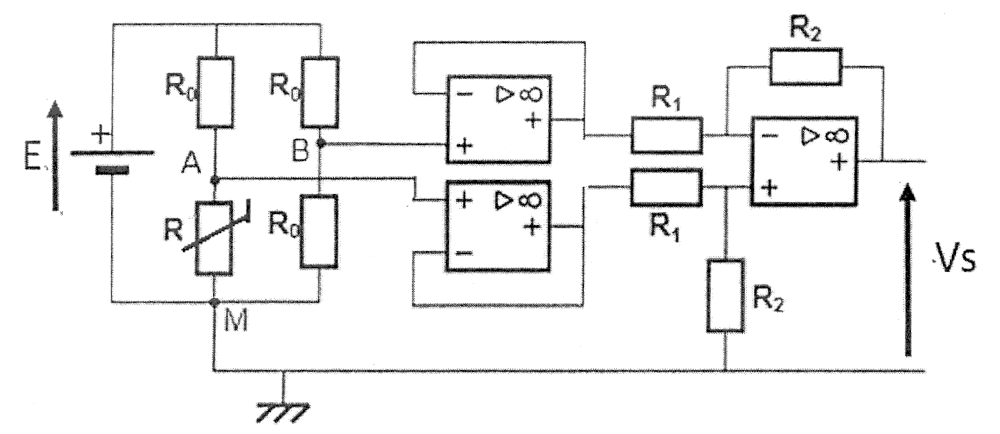
\includegraphics[width=0.8\linewidth]{./images/conditionneur-balance.png}
\end{figure}

\begin{enumerate}
    \item Déterminer l'expression de la tension $U_{AB} = f\left(E, K, m\right)$, sachant que $R = R_0 + \Delta R$ et $\frac{\Delta R}{R_0} = K.m$, m étant la masse à mesurer et K une constante.
    \item Calculer la valeur de la tension $U_{AB}$ pour $m = \SI{5}{\kilogram}$, si on a $R_0 = \SI{500}{\ohm}$, $K = 5.10^{-3} \si{\per\kilogram}$ et $E = \SI{12}{\volt}$.
    \item On admet qu'avec une masse $m < \SI{6}{\kilogram}$, on a le produit $K.m << 1$. Simplifier alors l'expression de $U_{AB}$ pour la rendre linéaire.
    \item On donne $R_1 = \SI{1}{\kilo\ohm}$. Calculer la valeur de $R_2$ pour obtenir $V_s = \SI{10}{\volt}$ lorsque $m = \SI{5}{\kilogram}$.
    \item Tracer la caractéristique de transfert $V_S = f(m)$.
\end{enumerate}

\subsection{Déterminer $U_{AB} = f\left(E, K, m\right)$}
\paragraph{}
Sachant que $R = R_0 + \Delta R$ et $\frac{\Delta R}{R_0} = K.m$, m étant la masse à mesurer et K une constante.
\paragraph{Expression de $U_A$}
$$U_A = \frac{E.R}{R + R_0} = \frac{E.(R_0 + \Delta R)}{R_0 + \Delta R + R_0} = \frac{E.(R_0 + \Delta R)}{2R_0 + \Delta R}$$

\paragraph{Expression de $U_B$}
$$U_B = \frac{E.R_0}{R_0 + R_0} = \frac{E}{2}$$

\paragraph{Expression de $U_{AB}$}
\begin{align*}
    U_{AB} & = U_A - U_B = \frac{E.(R_0 + \Delta R)}{2R_0 + \Delta R} - \frac{E}{2}\\
    U_{AB} & = \frac{2E.(R_0 + \Delta R)-E.(2R_0 + \Delta R)}{2(2R_0 + \Delta R)}\\
    U_{AB} & = \frac{E}{2}.\frac{2R_0 + 2\Delta R - 2R_0 - \Delta R}{2R_0 + \Delta R}\\
    U_{AB} & = \frac{E}{2}.\frac{\Delta R}{2R_0 + \Delta R}\\
    U_{AB} & = \frac{E}{2}.\frac{\frac{\Delta R}{R_0}}{\frac{2R_0 + \Delta R}{R_0}}\\
    U_{AB} & = \frac{E}{2}.\frac{K.m}{2 + K.m}\\
    U_{AB} & = \frac{E.K.m}{4 + 2K.m}\\
\end{align*}

\subsection{Calcul de $U_{AB}$ pour $m = \SI{5}{\kilogram}$}
\paragraph{}
Sachant que $R_0 = \SI{500}{\ohm}$, $K = 5.10^{-3} \si{\per\kilogram}$ et $E = \SI{12}{\volt}$.
$$U_{AB} = \frac{E.K.m}{4 + 2K.m} = \frac{12.5.10^{-3}.5}{4 + 2.5.10^{-3}.5} = 74,074 \si{\milli\volt}$$

\subsection{Simplification de l'expression de $U_{AB}$}
$$U_{AB} = \frac{E.K.m}{4}$$
\paragraph{}Pour $m = \SI{5}{\kilogram}$
$$U_{AB} =  \frac{E.K.m}{4} = \frac{12.5.10^{-3}.5}{4} = 75 \si{\milli\volt}$$

\subsection{Calcul de la valeur de $R_2$ pour obtenir $V_s = \SI{10}{\volt}$ lorsque $m = \SI{5}{\kilogram}$}
\paragraph{}Sachant que $R_1 = \SI{1}{\kilo\ohm}$.
\paragraph{}
Les deux premiers AOP sont monté en buffer et le dernier en soustracteur, on a donc : $$V_s = \frac{R_2}{R_1}(U_A-U_B) = \frac{R_2}{R_1}U_{AB}$$
\paragraph{}Calcul de $R_2$ :
$$R_2 = \frac{R_1.V_S}{U_AB} = \frac{10^3.10}{75.10^{-3}} = 133,33 \si{\kilo\ohm}$$

\subsection{Caractéristique de transfert}
$$V_s = \frac{R_2}{R_1}U_{AB} = \frac{R_2}{R_1}.\frac{E.K.m}{4} = \frac{133,33.10^{3}}{10^{3}}.\frac{12.5.10^{-3}m}{4}$$
$$V_s = 2m$$

\begin{figure}[H]
    \centering
    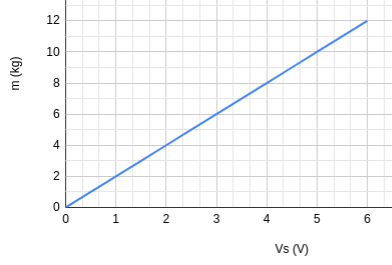
\includegraphics[width=0.5\linewidth]{./images/cond-balance-caract-transfert.png}
\end{figure}

\paragraph{} Pour $m = \SI{5}{\kilogram}$, on a bien $V_s = 2.5 = \SI{10}{\volt}$.

\subsection{Vérification avec Qucs}

\begin{figure}[H]
    \centering
    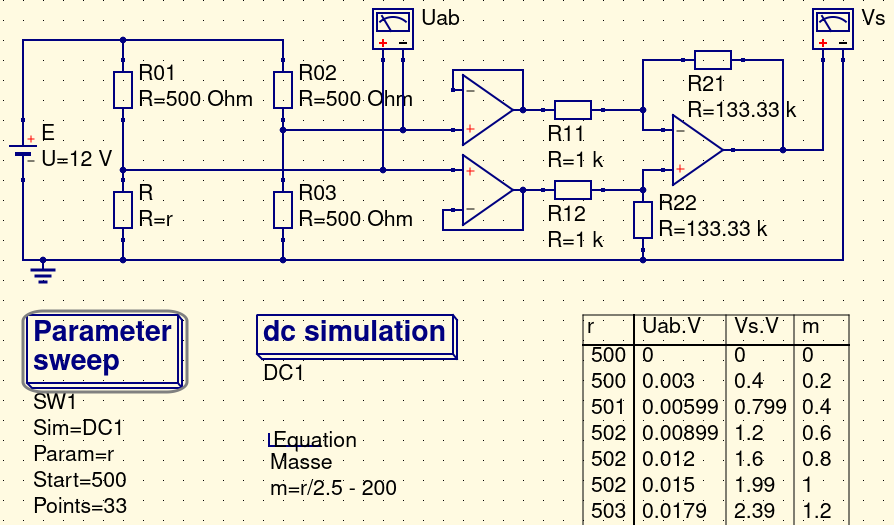
\includegraphics[width=0.9\linewidth]{./images/cond-balance-qucs.png}
\end{figure}

\begin{itemize}
    \item $R = R_0 + \Delta R \Rightarrow \Delta R = R - R_0$
    \item $\frac{\Delta R}{R_0} = K.m \Rightarrow m = \frac{\Delta R}{R_0.K} = \frac{R - R_0}{500.5.10^{-3}} = \frac{R}{2,5} - 200$
\end{itemize}

\paragraph{Vérification pour m = 5 kg :} en examinant la tableau suivant, on constate qu'une masse de 5kg correspond à une tension de sortie d'environ 10V (et à une tension AB de 74 mV).

\begin{figure}[H]
    \centering
    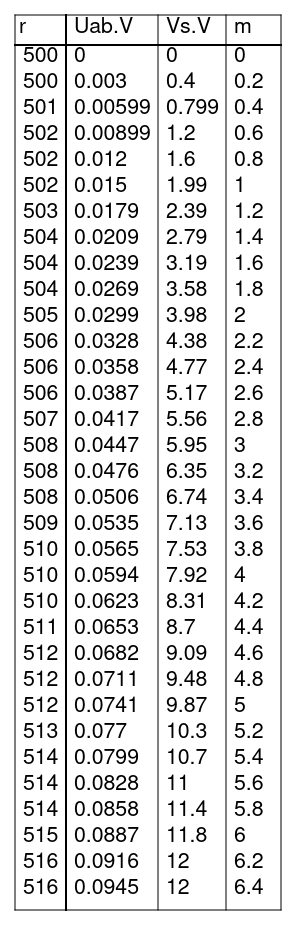
\includegraphics[width=0.3\linewidth]{./images/cond-balance-export.png}
\end{figure}


\newpage
\section{Circuits intégrés : 74LSxx et 74HCxx (13 janvier 2020)}
\paragraph{}
La famille 74LSxx possède les caractéristiques suivantes :
\begin{itemize}
    \item $V_{OHmin} = 2,4\si{\volt}$
    \item $V_{OLmax} = 0,4\si{\volt}$
\end{itemize}
\paragraph{}
La famille 74HCxx possède les caractéristiques suivantes :
\begin{itemize}
    \item $V_{IHmin} = 3,5\si{\volt}$
    \item $V_{ILmax} = 1\si{\volt}$
\end{itemize}
\paragraph{}
Peut-on raccorder l'entrée d'une porte 74HC avec la sortie d'une porte LS ? Dans l'affirmatif, calculer l'immunité aux bruits pour chaque niveau.

\paragraph{Réponse :}
\
Non car la tension de sortie à l'état haut minimale de la porte 74LS est inférieure à la tension d'entrée à l'état haut minimale de la porte 74HC : les valeurs ente 2,4 et 3,5 \si{\volt} seront perdues.

\paragraph{}A l'état LOW, la marge de bruit $M_L = V_{ILmax} - V_{OLmax} = 0,6 \si{\volt}$. A l'état HIGH, $M_H = V_{OHmin} - V_{IHmin} = -1,1 \si{\volt}$. Pour que le circuit fonctionne, ces deux valeurs auraient dû être positives.


\newpage
\section{Débitmètre (13 janvier)}
\paragraph{}
La mesure du débit d'une station de pompage est confiée à un débitmètre électromagnétique Promag 50H Endress+Hauser.

\paragraph{}\textbf{Extrait de la documentation technique :}
\begin{table}[H]
    \centering
    \begin{tabular}{l l}
        & \textbf{Grandeurs d'entrée}\\
    \hline
    \textbf{Grandeur de mesure} & Vitesse d'écoulement (proportionnelle à la tension induite)\\
    \hline
    \textbf{Gamme de mesure}    & Typique v = 0,01...10m/s avec la précision de mesure spécifiée\\
    \hline
    \textbf{Dynamique de mesure}& Supérieure à 1000 : 1\\
    \hline
    \textbf{Signal d'entrée}    & Entrée état (entrée auxiliaire) :\\
    & U = 3...30 V DC, $R_i = \SI{5}{\kilo\ohm}$, séparation galvanique.\\
    & Configurable pour : remise à zéro du/des totaliseur(s), suppression de la\\
    & mesure,  remise à zéro des messages défaut, démarrer/stopper un dosage.\\
    \\
        & \textbf{Grandeurs de sortie}\\
    \hline
    \textbf{Signal de sortie} & Promag 50\\
    & Sortie courant :\\
    & actif/passif au choix, séparation galvanique, constante de temps au choix \\
    & (0,05...100s), fin d'échelle réglable, coefficient de température : typ. 0,0005\% \\
    & de m/\si{\celsius}; résolution : 0,5\si{\micro\ampere} \\
    & -- actif : 0/4...20 mA, $R_c < 700\si{\ohm}$ (pour HART = $R_c \ge 250\si{\ohm}$)\\
    & -- passif : 0/4...20 mA, max. 30 V DC, $R_i \le 150\si{\ohm}$\\
\end{tabular}
\end{table}

\paragraph{}
Le capteur est inséré le long de la conduite PVC de refoulement, son orifice est de section égale à celle de la conduite, à savoir qu'il a un diamètre intérieur \textbf{D = 40mm}. Le débit est prévu pour fluctuer entre 2 et 20 $m^3/h$.

\paragraph{}
Le débitmètre renvoie l'information "débit Q" sur une sortie 4 - 20 mA. Cette information sera ensuite récupérée par une entrée analogique de l'automate après conversion en une tension $V_Q$ comprise entre \textbf{0 et 10 V}, conformément à la figure suivante. Le convertisseur 4-20 mA/0-10 V a une impédance d'entrée \textbf{$Z_e = \SI{600}{\ohm}$}.

\begin{figure}[H]
    \centering
    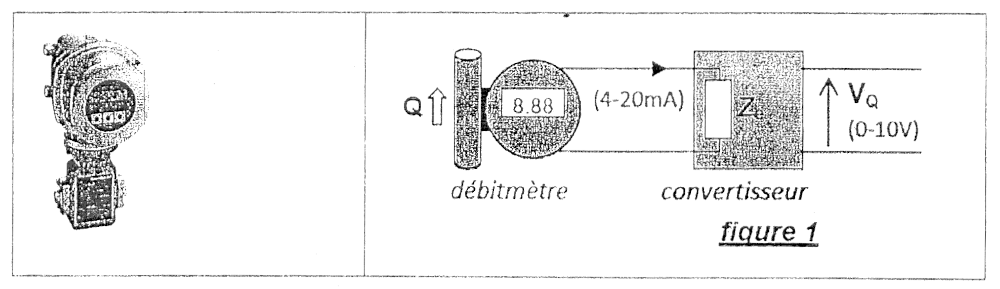
\includegraphics[width=\linewidth]{./images/debitmetre.png}
\end{figure}

\paragraph{}
On demande de
\begin{enumerate}
    \item déterminer la plage de débit mesurable par l'appareil et justifier son choix.
    \item calculer la tension maximale fournie par la sortie 4-20 mA du débitmètre. Cette valeur est-elle compatible avec les spécifications du constructeur du débitmètre ?
    \item calculer le facteur K tel que $\frac{\partial V_Q}{\partial Q} = K$, sachant que le débitmètre peut renvoyer une valeur Q au maximum égale à 70 $m^3/h$. Préciser son unité.
\end{enumerate}

\subsection{Calcul de la plage de débit}
Diamètre : $D = \SI{40}{\milli\meter} = 40.10^{-3}\si{\meter}$\\
Section : $S = \pi R^2 = \pi \left(\frac{D}{2}\right)^2 = \pi \left(\frac{4.10^{-2}}{2}\right)^2 = 4 \pi .10^{-4} = 1,257 \si{\milli\meter^2}$\\
Le débitmètre est prévu pour fonctionner entre 0,01 et 10 m/s.\\
\textbf{Débit minimum =} $0,01 . 1,257.10^{-3} = 1,257.10^{-5} \si{\meter}^3/\si{\second} = 1,257.10^{-5} . 3600 = 0,045 \si{\meter}^3/\si{\hour}$\\
\textbf{Débit maximum =} $10 . 1,257.10^{-3} = 1,257.10^{-2} \si{\meter}^3/\si{\second} = 1,257.10^{-2} . 3600 = 45 \si{\meter}^3/\si{\hour}$

\subsection{Calcul de la tension maximale}
$$V_{O max} = Z_e . I_{max} = 600.20.10^{-3} = 12 \si{\volt}$$

\subsection{Calcul de K}
$$K = \frac{\partial V_Q}{\partial Q} = \frac{10 - 0}{70 - 0} = 0,14 \si{\volt\hour}/\si{\meter^3}$$


\newpage
\section{AOP : exercice 1 (13 janvier 2020)}
\paragraph{}
Le schéma suivant représente un amplificateur à gain variable destiné pour les capteurs.
\begin{figure}[H]
    \centering
    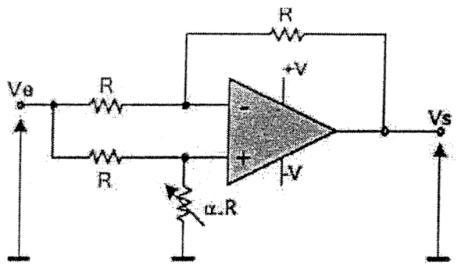
\includegraphics[width=0.4\linewidth]{./images/AOP1.png}
\end{figure}
\paragraph{}
Démontrer que : $$V_s = V_e \frac{\alpha - 1}{\alpha + 1}$$

\subsection{Démonstration}
L'amplificateur est monté en contre-réaction : $V+ = V-$.

\paragraph{}Expression de V+ (Millman) :
\begin{align*}
    V+ & = \frac{\frac{V_e}{R}+\frac{V_s}{R}}{\frac{1}{R}+\frac{1}{R}} \\
    V+ & = \frac{V_e + V_s}{2}                                         \\
\end{align*}

\paragraph{}Expression de V- (pont diviseur) :
\begin{align*}
    V- & = V_e\frac{\alpha R}{R + \alpha R} \\
    V- & = V_e\frac{\alpha}{1 + \alpha}   \\
\end{align*}

\paragraph{}Expression de $V_s$ :
\begin{align*}
    V+                  & = V-                              \\
    \frac{V_e + V_s}{2} & = \frac{V_e.\alpha}{1 + \alpha}   \\
    V_s & = \frac{2V_e.\alpha}{1 + \alpha} - V_e            \\
    V_s & = V_e.\frac{2\alpha - 1 - \alpha}{1 + \alpha}     \\
    V_s & = V_e.\frac{\alpha - 1}{1 + \alpha}     \\
\end{align*}

\subsection{Vérification avec Qucs}

\begin{figure}[H]
    \centering
    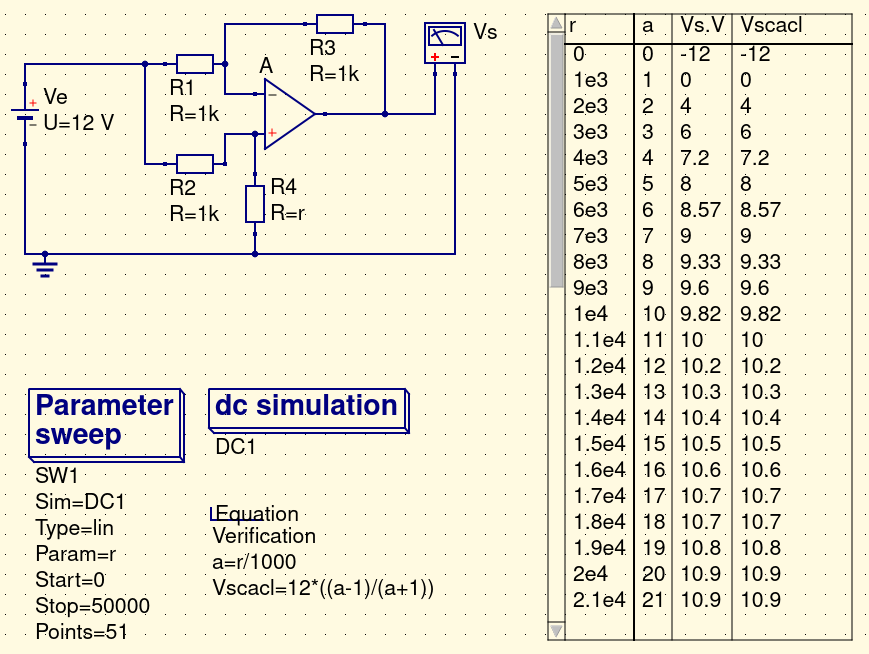
\includegraphics[width=0.95\linewidth]{./images/AOP1-res.png}
\end{figure}

\paragraph{}La tension de sortie mesurée ($V_s$) correspond bien à la tension de sortir calculée ($V_{scalc}$).

\newpage
\section{AOP : exercice 2 (13 janvier 2020)}
\paragraph{}
On désire amplifier et adapter la tension $V_e$ fournie par un capteur de température. Pour cela, on utilise le montage amplificateur différenciateur suivant :
\begin{itemize}
    \item AOP est considéré idéal
    \item $V_{ref} = \SI{2.73}{\volt}$
    \item $V = \SI{12}{\volt}$
    \item $T(\si{\celsius}) = T(\degree\si{\kelvin}) - 273\degree\si{\kelvin}$
\end{itemize}
\begin{figure}[H]
    \centering
    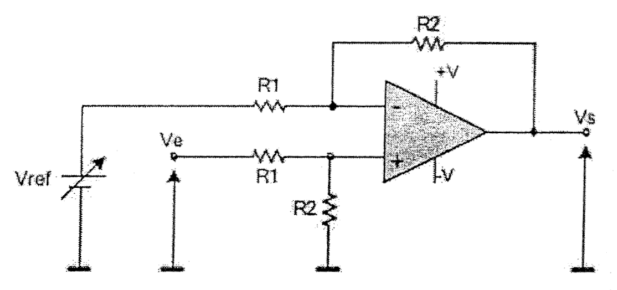
\includegraphics[width=0.5\linewidth]{./images/AOP2.png}
\end{figure}

\begin{enumerate}
    \item Exprimer la tension $V_s$ en fonction de $R_1$, $R_2$, $V_{ref}$ et $V_e$.
    \item Sachant que le capteur de température fournit une tension de \SI{10}{\milli\volt} pour 1\degree\si{\kelvin}, calculer le rapport $\frac{R_2}{R_1}$ pour qu'à la sortie de l'amplificateur, $V_S = \SI{20}{\milli\volt}$ pour \SI{1}{\celsius}.
\end{enumerate}

\subsection{Expression de $V_s$}
\paragraph{}L'AOP est monté en soustracteur :
$$V_s = \frac{R_2}{R_1}\left(V_e - V_{ref}\right)$$

\subsection{Calcul du rapport R2/R1}
\paragraph{} Calcul de $V_e$ pour \SI{1}{\celsius} :

$$1\si{\celsius} = 1 + 273 = 274\si{\kelvin}$$
\begin{align*}
    \SI{1}{\kelvin} &\to \SI{10}{\milli\volt}\\
    \SI{274}{\kelvin} = \SI{1}{\celsius} &\to \SI{2.74}{\volt}\\
\end{align*}

\paragraph{} Calcul du gain $\frac{R_2}{R_1}$ :
\begin{align*}
    V_s &= \frac{R_2}{R_1}\left(V_e - V_{ref}\right)\\
    \frac{R_2}{R_1} &= \frac{V_s}{V_e - V_{ref}}\\
    \frac{R_2}{R_1} &= \frac{20.10^{-3}}{2.74 - 2.73}\\
    \frac{R_2}{R_1} &= 2\\
\end{align*}

\subsection{Vérification avec Qucs}

\begin{figure}[H]
    \centering
    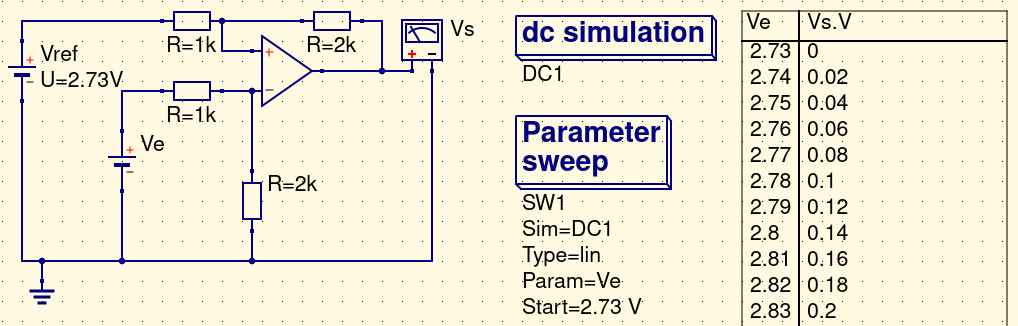
\includegraphics[width=\linewidth]{./images/AOP2-res.png}
\end{figure}


\newpage
\section{Amplificateur d'instrumentation (13 janvier 2020)}
\paragraph{}
Le montage ci-dessous représente un amplificateur différentiel utilisé dans les instruments de mesure pour les faibles tensions continues issues d'un capteur :
\begin{figure}[H]
    \centering
    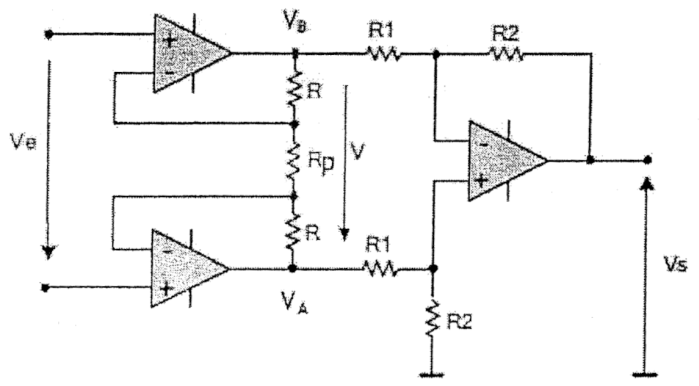
\includegraphics[width=0.6\linewidth]{./images/AOP3.png}
\end{figure}

\begin{enumerate}
    \item Sachant que les 3 AOP sont idéaux, exprimer la tension V en fonction de l'entrée $V_e$.
    \item Exprimer la tension $V_s$ en fonction de $V_A$, $V_B$, $R_1$ et $R_2$.
    \item Déduire l'expression de $V_s$ en fonction de V, puis de $V_s$ en fonction de $V_e$.
\end{enumerate}

\subsection{Expression de V}
\paragraph{}Expression de V+ de AOP1 (en haut à gauche) :
$$V+ = 0$$

\paragraph{}Expression de V- de AOP1 (Millman) :
\begin{align*}
    V- &= \frac{ \frac{V_B}{R} + \frac{V_e}{R_p} } { \frac{1}{R} + \frac{1}{R_p} }\\
    V- &= \frac{ V_B.R_p + V_e.R } { R + R_p }\\
\end{align*}

\paragraph{}Expression de $V_B$ (AOP1 est en régime linéaire) :
\begin{align*}
    V+ &= V-\\
    0 &= \frac{ V_B.R_p + V_e.R } { R + R_p }\\
    V_B &= -\frac{V_e.R}{R_p}\\
\end{align*}

\paragraph{}Expression de V+ de AOP2 (en bas à gauche) :
$$V+ = V_e$$

\paragraph{}Expression de V- de AOP2 (Millman):
\begin{align*}
    V- &= \frac{ \frac{V_A}{R} } { \frac{1}{R} + \frac{1}{R_p} }\\
    V- &= \frac{V_A}{R} . \frac{R.R_p}{R + R_p}\\
    V- &= \frac{V_A.R_p}{R + R_p}\\
\end{align*}

\paragraph{}Expression de $V_A$ (AOP1 est en régime linéaire) :
\begin{align*}
    V+ &= V-\\
    V_e &= \frac{V_A.R_p}{R + R_p}\\
    V_A &= \frac{V_e(R + R_p)}{R_p}\\
\end{align*}

\paragraph{}Expression de V
\begin{align*}
    V &= V_A - V_B\\
    V &= \frac{V_e(R + R_p)}{R_p} + \frac{V_e.R}{R_p} \\
    V &= \frac{V_e}{R_p} \left(R + R_p + R\right) \\
    V &= \frac{V_e(2R + R_p)}{R_p} \\
\end{align*}

\subsection{Expression de $V_s$ en fonction de $V_A$, $V_B$, $R_1$ et $R_2$}

\paragraph{}Expression de V+ de AOP3 (à droite) :
\begin{align*}
    V+ &= \frac{ \frac{V_A}{R_1} } { \frac{1}{R_1} + \frac{1}{R_2} }\\
    V+ &= \frac{V_A}{R_1} . \frac{R_1.R_2}{R_1 + R_2}\\
    V+ &= \frac{V_A.R_2}{R_1 + R_2}\\
\end{align*}

\paragraph{}Expression de V- de AOP3 :
\begin{align*}
    V- &= \frac{ \frac{V_B}{R_1} + \frac{V_s}{R_2} } { \frac{1}{R_1} + \frac{1}{R_2} }\\
    V- &= \frac{ V_B.R_2 + V_s.R_1 } { R_1 + R_2 }\\
\end{align*}

\paragraph{}Expression de $V_s$
\begin{align*}
    V+ &= V-\\
    \frac{V_A.R_2}{R_1 + R_2} &= \frac{ V_B.R_2 + V_s.R_1 } { R_1 + R_2 } \\
    V_s &= \frac{V_A.R_2 - V_B.R_2}{R_1} \\
    V_s &= \frac{R_2}{R_1}(V_A - V_B) \\
\end{align*}

\subsection{Expression de $V_s$ en fonction de de V puis de $V_e$}
\begin{align*}
    V_s &= \frac{R_2}{R_1}V \\
    V_s &= \frac{R_2}{R_1}.\frac{V_e(2R + R_p)}{R_p} \\
    V_s &= V_e\frac{R_2}{R_1}\left(\frac{2R}{R_p} + \frac{R_p}{R_p}\right) \\
    V_s &= V_e\frac{R_2}{R_1}\left(\frac{2R}{R_p} + 1\right) \\
\end{align*}

\subsection{Vérification avec Qucs}
\paragraph{}
Avec R = \SI{1}{\kilo\ohm}, $R_p$ = \SI{500}{\ohm}, $R_1$ = \SI{1}{\kilo\ohm} et $R_2$ = \SI{2}{\kilo\ohm}

\begin{align*}
    V_s &= V_e\frac{2000}{1000}\left(\frac{2.1000}{500} + 1\right)\\
    V_s &= 10V_e
\end{align*}

\begin{figure}[H]
    \centering
    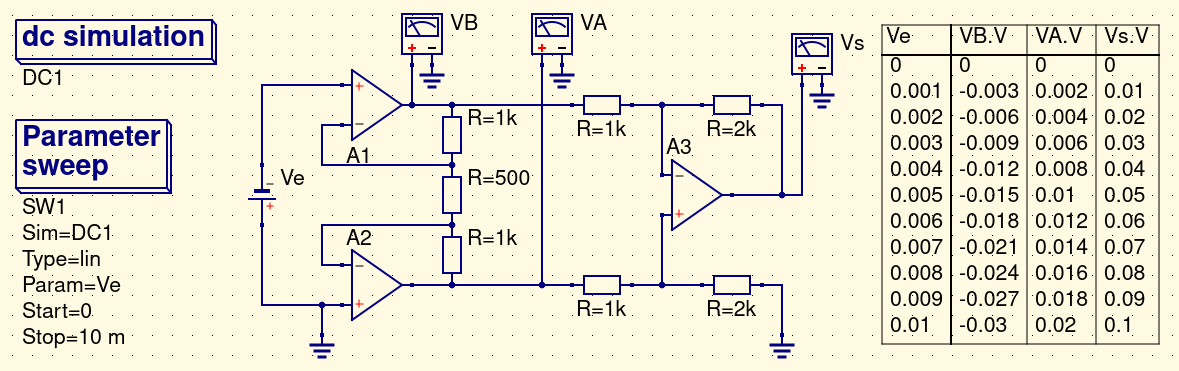
\includegraphics[width=\linewidth]{./images/AOP3-res.png}
\end{figure}

\paragraph{}
Pour une tension d'entrée de 0 à 10 mV, les résultats sont bien corrects.


\newpage
\section{Aimants : exercice 1 (20 janvier 2020)}
\paragraph{}
Une bobine de 5cm de diamètre, longue de 45cm comprend 500 spires en fil de cuivre de 0,4mm de diamètre. Elle est traversée par un courant de 320mA.

\paragraph{}
Calculer
\begin{enumerate}
    \item L'intensité du champ magnétique au centre de cette bobine.
    \item La valeur de l'induction.
    \item Le flux magnétique produit.
\end{enumerate}

\subsection{Intensité du champ magnétique}
\begin{align*}
    B &= \mu_0.\frac{N}{l}.I\\
    B &= \frac{4 \pi 10^{-7}.500.320.10^{-3}}{45.10^{-2}}\\
    B &= 446,804 \si{\micro\tesla}\\
\end{align*}

\subsection{Induction (champ d'excitation magnétique)}
\begin{align*}
    H &= \frac{N}{l}.I\\
    H &= \frac{500.320.10^{-3}}{45.10^{-2}}\\
    H &= 335,556 \si{\ampere}/\si{\meter}\\
\end{align*}

\subsection{Flux magnétique}
\begin{align*}
    \Phi &= \overrightarrow{B}.\overrightarrow{S} = B.S.\cos\theta\\
    \Phi &= B\pi\left(\frac{d}{2}\right)^2\\
    \Phi &= 446,804.10^{-6}\pi\left(2,5.10^{-2}\right)^2\\
    \Phi &= 877,298 \si{\nano\weber}\\
\end{align*}

\newpage
\section{Aimants : exercice 2 (20 janvier 2020)}
\paragraph{}
Une bobine de 2cm de diamètre comprend 1200 spires en fil de cuivre de diamètre de 0,5mm de diamètre. On place à l'intérieur de cette bobine un noyau ferromagnétique de perméabilité relative égale à 500. On alimente cette bobine au moyen d'une source de tension dont la FEM E = 6V et la résistance interne R = 2,2 \si{\ohm}.

\paragraph{}
Calculer
\begin{enumerate}
    \item L'intensité du champ magnétique au centre de cette bobine.
    \item La valeur de l'induction.
    \item La valeur du flux magnétique produit.
\end{enumerate}

\subsection{Intensité du champ magnétique}
$L_{fil} = 2 \pi \frac{d_{spire}}{2}N_{spires} = 2 \pi \frac{2.10^{-2}}{2}1200 = 75,398 \si{\meter}$\\
$S_{fil} = \pi \left(\frac{d_{fil}}{2}\right)^2 = \pi \left(\frac{5.10^{-4}}{2}\right)^2 = 196,35 \si{\nano\meter^2}$\\
$R_{fil} = \rho_{Cu} \frac{L_{fil}}{S_{fil}} = 17.10^{-9} \frac{75,398}{196,35.10^{-9}} = 6,528 \si{\ohm}$\\
$I = \frac{E}{R + R_{fil}} = \frac{6}{2,2 + 6,528} = 687,443\si{\milli\ampere}$\\
$l_{bobine} = d_{fil}.N_{spires} = 5.10^{-4}.1200 = 0,6\si{\meter}$
$$B = \mu_0.\mu_r\frac{N.I}{l_{bobine}} = \frac{4\pi10^{-7}.500.1200.687,443.10^{-3}}{0,6} = 863,866 \si{\milli\tesla}$$

\subsection{Induction (champ d'excitation magnétique)}
$$H = \frac{N.I}{l} = \frac{1200.687,443.10^{-3}}{0,6} = 1,375 \si{\kilo\ampere}/\si{\meter}$$

\subsection{Flux magnétique}
$$ \Phi= B.S.\cos\theta = 863,866.10^{-3}\pi10^{-4} = 271,392 \si{\micro\weber}$$


\newpage
\section{Thermocouple : résumé (27 janvier 2020)}
\paragraph{}
Résumer le document \emph{doc4-thermocouple-guide.pdf}.

\subsection{Définition}
\paragraph{}
Un thermocouple est un transducteur de chaleur : il transforme une température en un signal électrique.

\subsection{Principe de fonctionnement}
\paragraph{}
Le thermocouple fonctionne grâce à l'effet de Seebeck : lorsque deux métaux de nature différente sont mis en contact en circuit ouvert, une tension (tension de Seebeck) apparaît aux bornes du circuit. Cette tension est proportionnelle à la température et au c\oe fficient de Seebeck (qui lui-même varie en fonction de la température et rend donc la tension de sortie non linéaire sur de larges plages de mesure) selon l'équation : $$\Delta V \approx S \Delta T$$

\subsection{Types de thermocouples}
\paragraph{}
Il existe différent types de thermocouples désignés par une lettre majuscule en fonction du couple de matériaux qui les compose. Ces types sont réglementés par des normes ANSI.

\subsection{Jonctions isothermes et compensation de soudure froide}
\paragraph{}
Le thermocouple est composé de trois jonctions : la jonction des deux métaux (J1) et les jonctions de chacun des deux à la carte d'acquisition (J2 et J3). J2 et J3 produisent elles aussi une tension qu'il faudra soustraire à la tension de J1 pour obtenir la température de J1. Pour ce faire, elles sont maintenues à la même température : elles produisent donc des tensions de valeur égale et de signe opposé qui s'annulent.

\begin{figure}[H]
    \centering
    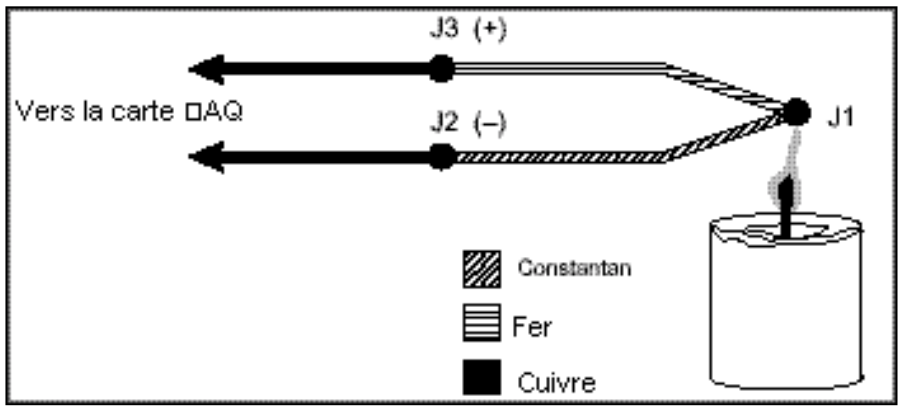
\includegraphics[width=0.6\linewidth]{./images/thermocouple1.png}
\end{figure}

\paragraph{}
Pour éliminer les tensions parasites, on utilise une soudure froide (traditionnellement maintenue à 0\si{\celsius}) dont la tension servira de référence : lorsque $T_1 > T_{ref}$, la tension de sortie est positive et dans le cas contraire, elle est négative.

\begin{figure}[H]
    \centering
    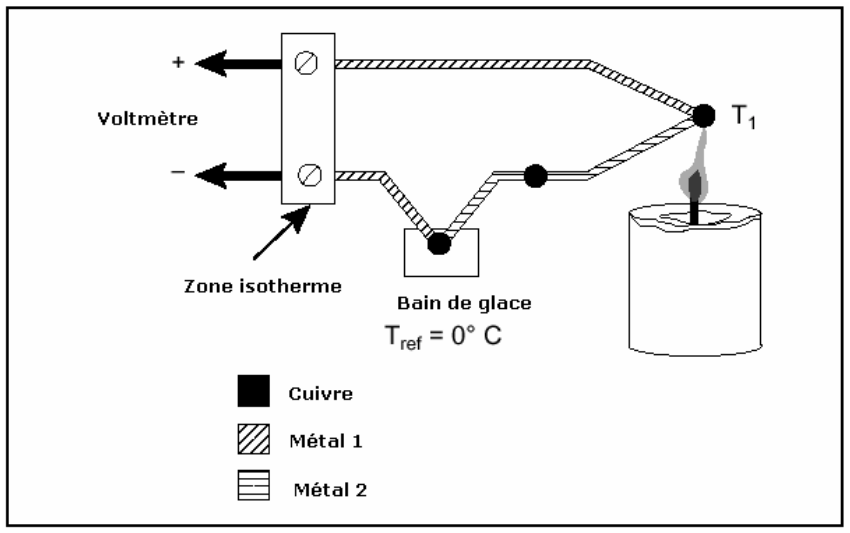
\includegraphics[width=0.6\linewidth]{./images/thermocouple2.png}
\end{figure}

\paragraph{}
En pratique, la soudure de référence n'est pas nécessairement maintenue à \SI{0}{\celsius} (car c'est peu pratique) : elle est soit connue, soit mesurée par un capteur de température à lecture directe pour pouvoir soustraire sa tension à la tension fournie par la jonction dont on souhaite connaître la température (c'est la compensation logicielle). Une compensation matérielle est également possible en ajoutant une source de tension qui varie en fonction de la température ambiante et permet d'annuler les tensions parasites. La compensation matérielle est moins précise que la compensation logicielle et nécessite que chaque type de thermocouple ait son propre circuit de compensation (ce qui rend cher le circuit).

\subsection{Tables de conversion}
\paragraph{}
Il est nécessaire d'utiliser une soudure de référence car les tables de référence NIST sont établies par rapport à une soudure froide (\SI{0}{\celsius}). Ces tables de conversion sont nécessaires car le signal de sortie d'un thermocouple n'est pas linéaire sur de larges plages de températures mesurées.


\subsection{Conditionnement du signal}
\paragraph{}
Les thermocouples nécessitent un conditionnement particulier du signal pour amplifier et filtrer la tension de sortie, par exemple de type SCXI (Signal Conditioning eXtensions for Instrumentation). En effet, le thermocouple ne peut pas être connecté directement à un circuit de sortie car le fait de connecter les fils du thermocouple au système de
mesure crée des circuits thermo-électriques supplémentaires. De plus, les signaux des thermocouples ont une forte sensibilité aux bruits : le niveau du bruit est souvent supérieur ou égal au signal du thermocouple.

\subsection{Avantages}
\begin{itemize}
    \item prix avantageux
    \item plage de température large
\end{itemize}

\subsection{Inconvénients}
\begin{itemize}
    \item nécessité d'une compensation de soudure froide (compensation logicielle le plus souvent)
    \item signal de sortie non linéaire sur de larges plages de mesure(nécessité d'une table de conversion)
    \item signal de sortie sensible aux bruits (nécessité d'un conditionnement particulier du signal : câbles blindés, amplification, filtrage d'entrée)
    \item ajout conseillé d'une détection de thermocouple ouvert
\end{itemize}


%\section{Recherches sur le RS 485 (3 février)}
%\section{Indices de protection (3 février)}

\newpage
\section{Conditionneur : exercice 2 (3 février 2020)}
\paragraph{}
Le montage suivant utilise 4 AO que l'on supposera idéaux. Une sonde de platine est insérée dans la boucle de réaction de l'AO1.

\paragraph{}
$V_Z = 1,2\si{\volt}$ et $V_{cc} = 15\si{\volt}$.

\paragraph{}
$R_3 = R_4 = R_5 = 100\si{\ohm}$, $R_2 = R_6 = R_7 = 1\si{\kilo\ohm}$ et $R_8 = R_9$

\begin{figure}[H]
    \centering
    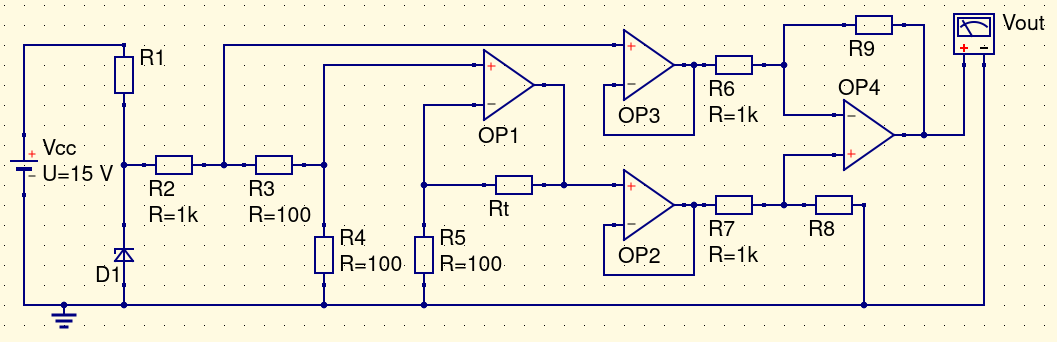
\includegraphics[width=\linewidth]{./images/cond2.png}
\end{figure}

\begin{enumerate}
    \item Décomposer ce circuit en différents étages et expliquer le rôle de chacun.
    \item Exprimer la tension de sortie Vs en fonction de R(T).
    \item Ce montage peut-il fonctionner avec des AO mono tensions (c’est-à-dire alimentés entre 0\si{\volt} et $V_{cc}$)?
\end{enumerate}

\subsection{Décomposer le circuit}
\begin{itemize}
    \item $D_1$ et $R_1$ servent à stabiliser la tension
    \item $OP_1$ est monté en non inverseur : $V_s = V_e\left(1 + \frac{R_T}{R_5}\right)$
    \item $OP_2$ et $OP_3$ sont montés en buffers : $V_s = V_e$
    \item $OP_4$ est monté en soustracteur = $V_s = \frac{R_{8/9}}{R_{6/7}}(V_{(+)} - V_{(-)})$
\end{itemize}

\subsection{Expression de $V_s$}
\begin{align*}
    &V_{s OP3} = V_{R34} = \frac{V_Z(R_3 + R_4)}{R_2 + R_3 + R_4} = \frac{1,2.200}{1200} = 200 \si{\milli\volt}\\
    &V_{s OP2} = V_{s OP1} = V_{R4} \left(1 + \frac{R_T}{R_5}\right)= \frac{V_Z.R_4}{R_2 + R_3 + R_4} \left(1 + \frac{R_T}{R_5}\right) = \frac{1,2.100}{1200} \left(1 + \frac{R_T}{100}\right) = 0,1 + R_T . 10^{-3}\\
    & V_{s} = V_{s OP4} = \frac{R}{R_{6/7}}\left(V_{s OP2} - V_{s OP3}\right) = R.R_T.10^{-6} - R.10^{-4}
\end{align*}
Avec $R = R_8 = R_9$

\subsection{Ce montage peut-il fonctionner avec des AOP mono tensions ?}
$V_{sOP3} > 0$ $(= 0,2 \si{\volt})$ et $V_{sOP2} > 0$ $(= 0,1 + R_T . 10^{-3})$ et $R_T > 0$). La seule condition pour pouvoir utiliser des AOP mono tensions est que $V_{sOP2} > V_{sOP3}$ :
\begin{align*}
    0,1 + R_T . 10^{-3} &> 0,2\\
    R_T &> 100\si{\ohm}\\
\end{align*}

\subsection{Vérification avec Qucs}
\begin{align*}
    & R_8 = R_9 = 2 \si{\kilo\ohm}\\
    & R_{T min} = 0 \si{\ohm}*\\
    & R_{T max} = \frac{V_{cc max} + R.10^{-4}}{R.10^{-6}} = \frac{15 + 0,2}{2.10^{-3}} = 7600 \si{\ohm}\\
\end{align*}
* $> 100 \si{\ohm}$ si $V_{cc min} = 0$

\begin{figure}[H]
    \centering
    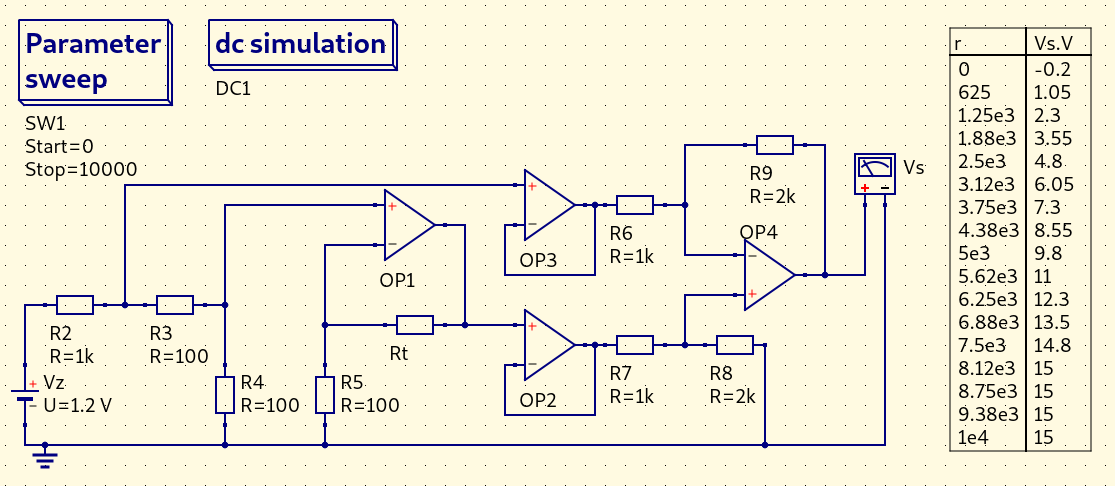
\includegraphics[width=\linewidth]{./images/cond2-qucs.png}
\end{figure}

\paragraph{}
Pour $R_T \ge 7,6\si{\kilo\ohm}$, $V_s$ est saturé à $V_{cc max} = 15 \si{\volt}$ :
\begin{figure}[H]
    \centering
    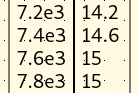
\includegraphics[width=0.15\linewidth]{./images/cond2-rtmax.png}
\end{figure}

\paragraph{}
Pour $R_T \le 100\si{\ohm}$, $V_s < 0\si{\volt}$ :
\begin{figure}[H]
    \centering
    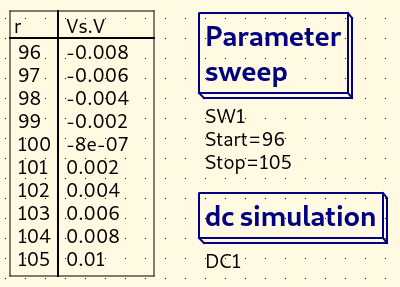
\includegraphics[width=0.4\linewidth]{./images/cond2-monotension.png}
\end{figure}

\paragraph{}
Caractéristique de transfert :
\begin{figure}[H]
    \centering
    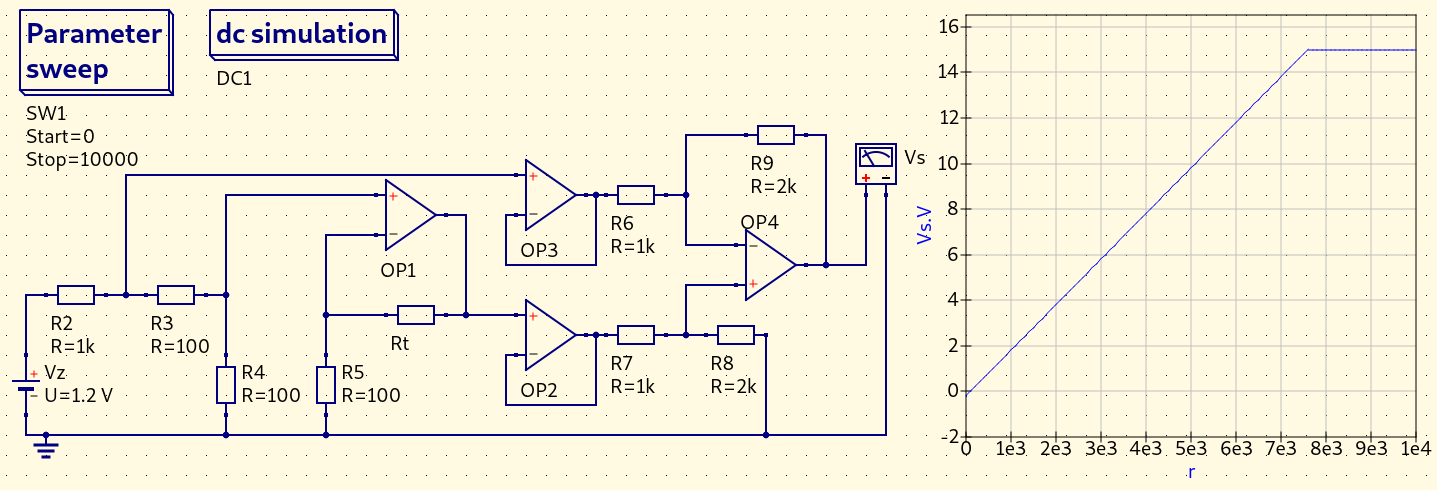
\includegraphics[width=\linewidth]{./images/cond2-caract-transfert.png}
\end{figure}
\paragraph{}
La tension de sortie est négative pour les première valeurs de $R_T$ et est saturée à \SI{15}{\volt} lorsque $R_T$ est supérieure à 7,6\si{\kilo\ohm}.

\newpage
\section{Pont de Wheatstone : conditionnement de la jauge de contrainte (10 février 2020)}
\paragraph{}
Montrer que
$$V_O = V_I \left[\frac{R_3}{R_3 + R_g} - \frac{R_2}{R_1 + R_2}\right]$$
\paragraph{}
et que, à $V_O = 0\si{\volt}$,
$$\frac{R_1}{R_4} = \frac{R_2}{R_3}$$

\begin{figure}[H]
    \centering
    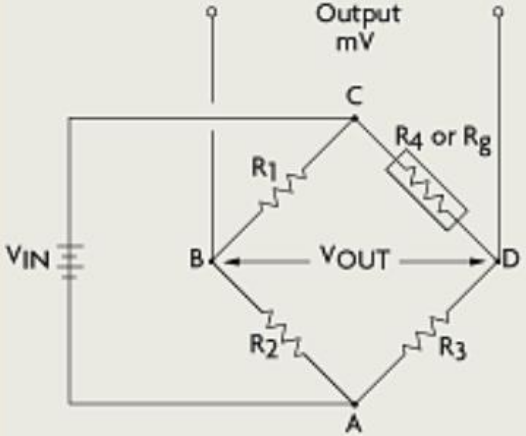
\includegraphics[width=0.4\linewidth]{./images/wheatstone.png}
\end{figure}

\subsection{Démonstration}
\begin{align*}
    V_D &= V_I\frac{R_g}{R_3 + R_g}\\
    V_B &= V_I\frac{R_2}{R_1 + R_2}\\
    V_O &= V_D - V_B\\
    V_O &= V_I \left[\frac{R_3}{R_3 + R_g} - \frac{R_2}{R_1 + R_2}\right]\\
\end{align*}

\begin{align*}
    &V_I \left[\frac{R_3}{R_3 + R_4} - \frac{R_2}{R_1 + R_2}\right] = 0\\
    &\frac{R_3}{R_3 + R_4} - \frac{R_2}{R_1 + R_2} = 0\\
    &R_3(R_1 + R_2) - R_2(R_3 + R_4) = 0\\
    &R_3R_1 + R_3R_2 - R_2R_3 - R_2R_4 = 0\\
    &R_3R_1 - R_2R_4 = 0\\
    &R_3R_1 = R_2R_4\\
    &\frac{R_1}{R_4} = \frac{R_2}{R_3}\\
\end{align*}



\newpage
\section{Capteurs de force (10 février 2020)}
\paragraph{}
Sur base du document doc3-Force-guide.pdf, répondre aux questions suivantes :
\begin{enumerate}
    \item Définir un capteur de force
    \item Comparer charge nominale et force de travail admissible
    \begin{enumerate}
        \item Comparer répétabilité et reproductibilité
        \item Comparer linéarité et hystérésis
        \item Définir la dérive thermique
    \end{enumerate}
    \item Jauge de contrainte
    \begin{enumerate}
        \item De quoi se compose une jauge de contrainte ? Comment l’utilise-t-on ?
        \item Permet-elle de travailler en compression et en traction ?
        \item Quelles sont les précisions atteintes ?
        \item Quelle est la gamme des forces mesurables ?
        \item Que se passe-t-il si le capteur passe en déformation plastique irréversible ?
    \end{enumerate}
    \item La tension renseignée dans le schéma ci-dessous est-elle correcte ?
    \begin{figure}[H]
        \centering
        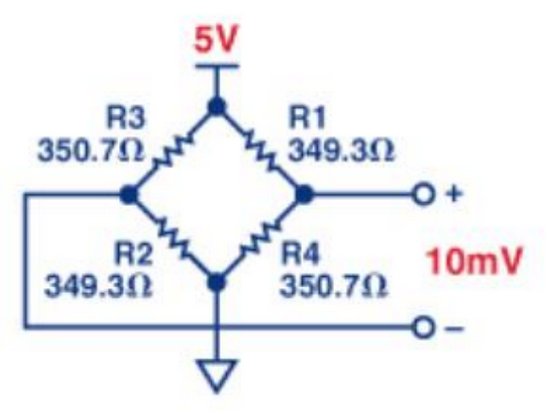
\includegraphics[width=0.3\linewidth]{./images/capteur-force-scaime-schema.png}
    \end{figure}
    \begin{enumerate}
        \item Faut-il utiliser un câble blindé pour raccorder le capteur ? Pourquoi ?
        \item Comment se comporte la résistance d’une jauge de contrainte si on l’étire ? Existe-t-il une direction privilégiée sur le capteur pour la mesure d’une force ?
    \end{enumerate}
    \item Quel est le but du conditionneur associé au capteur ? Donner 3 exemples
    \item Un capteur MS0x-5KN, 5mV/V est alimenté en 12V. Quelle est la force mesurée, si la tension délivrée par le capteur est de 30mV ?
    \begin{enumerate}
        \item Comment vérifie-t-on le bon fonctionnement du pont de Wheatstone ?
    \end{enumerate}
    \item Sur le site du constructeur
    \begin{enumerate}
        \item Comment peut-on choisir son capteur sur un axe dynamométrique ?
        \item Donner la signification de IP65, IP67, IP68 ?
        \item Expliquer les données de la figure suivante
    \end{enumerate}
\end{enumerate}

\begin{figure}[H]
    \centering
    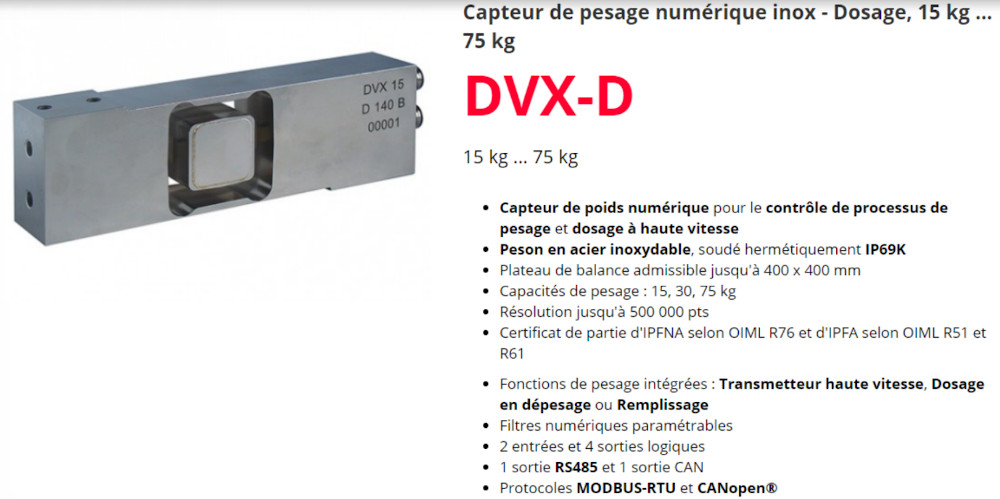
\includegraphics[width=\linewidth]{./images/capteur-force-scaime.jpg}
\end{figure}

\subsection{Définir un capteur de force}
\paragraph{}
Un capteur de force mesure une force en transformant un effort mécanique en un signal électrique proportionnel à cet effort.

\subsection{Comparer charge nominale et force de travail admissible}
\paragraph{}
La charge nominale est la force maximale que puisse mesurer le capteur (sans perte de données et sans détériorer le capteur). La force de travail admissible est la force maximale qui puisse être appliquée temporairement au capteur sans dérives permanentes (garantit seulement la non détérioration du capteur, pas la donnée). La force de travail admissible s'exprime en pourcentage de la charge nominale.

\subsubsection{Comparer répétabilité et reproductibilité}
\paragraph{}
La répétabilité est la différence maximale du signal pour des mesures effectuées dans des conditions similaires (le capteur est gardé dans la même position et l'environnement est le même). La reproductibilité désigne la différence maximale du signal dans des conditions différentes (l'environnement reste le même mais pas la position du capteur). La répétabilité et la reproductibilité sont exprimées en pourcentage du signal nominal.

\subsubsection{Comparer linéarité et hystérésis}
\paragraph{}
La linéarité désigne l'écart maximal du signal par rapport à la droite idéale (qui passe par zéro). L'hystérésis désigne la différence maximale du signal pour une même force entre la valeur lue en augmentant la force et la valeur lue en la diminuant la force. La linéarité et l'hystérésis sont exprimées en pourcentage du signal nominal.

\subsubsection{Définir la dérive thermique}
\paragraph{}
La dérive thermique désigne la variation du signal pour une même force lorsqu'on fait varier la température. Elle est exprimée en pourcentage de la charge nominale par degré Celsius.

\subsection{Jauge de contrainte}
\subsubsection{De quoi se compose une jauge de contrainte ? Comment l’utilise-t-on ?}
\paragraph{}
Une jauge de contrainte se compose d'un composant résistif gravé sur une "feuille" souple collée sur le corps du capteur. La valeur ohmique du composant résistif est modifiée lorsque la feuille est soumise à une compression ou à un étirement. Le capteur se compose de 4 (ou d'un multiple de 4) jauges de contraintes montées en pont de Wheatstone.

\subsubsection{Permet-elle de travailler en compression et en traction ?}
\paragraph{}
Oui

\subsubsection{Quelles sont les précisions atteintes ?}
\paragraph{}
$\pm0,1\% et \pm0,05\%$


\subsubsection{Quelle est la gamme des forces mesurables ?}
\paragraph{}
De quelques N à plusieurs MN


\subsubsection{Que se passe-t-il si le capteur passe en déformation plastique irréversible ?}
\paragraph{}
Les jauges de contrainte ne peuvent plus revenir à leur état initial lorsqu'il n'est plus soumis à une force. La capteur n'est plus calibré correctement : le signal est décalé et peut continuer à se décaler même sans que le capteur soit encore soumis à une force dépassant la force de travail admissible. Le capteur ne peut donc pas être recalibré : il peut être jeté.

\subsection{La tension renseignée dans le schéma est-elle correcte ?}
\begin{align*}
    V_s &= V_e\left(\frac{R_4}{R_1 + R_4} - \frac{R_2}{R_2 + R_3}\right)\\
    V_s &= 5\left(\frac{350.7 - 349.3}{700}\right)\\
    V_s &= \SI{10}{\milli\volt}\\
\end{align*}

\subsubsection{Faut-il utiliser un câble blindé pour raccorder le capteur ? Pourquoi ?}
\paragraph{}
Oui car les signaux de sortie sont très faibles (variations de quelques millivolts).

\subsubsection{Comment se comporte la résistance d’une jauge de contrainte si on l’étire ? Existe-t-il une direction privilégiée sur le capteur pour la mesure d’une force ?}
\paragraph{}
Un axe standard mesure une force dans une seule direction. Cette direction doit être respectée pour éviter les erreurs de mesure (ou éventuellement l'endommagement du capteur).

\subsection{Quel est le but du conditionneur associé au capteur ? Donner 3 exemples}
Le but est d'amplifier et de filtrer le signal du capteur qui est très faible ainsi que de fournir une alimentation très stable au capteur.

\paragraph{}
Exemples :
\begin{itemize}
    \item Transmetteur analogique à sortie analogie ou numérique : le signal est modifié et transmis.
    \item Afficheur : le signal est affiché et peut aussi être transmis.
    \item Centrale d'acquisition : permet de rassembler plusieurs signaux pour le contrôle de process (ces signaux peuvent aussi être enregistrés sur carte SD).
\end{itemize}

\subsection{Un capteur MS0x-5KN, 5mV/V est alimenté en 12V. Quelle est la force mesurée, si la tension délivrée par le capteur est de 30 mV ?}
\paragraph{}
2,5 \si{\kilo\newton}

\subsubsection{Comment vérifie-t-on le bon fonctionnement du pont de Wheatstone ?}
Les résistances entre les différentes sorties comme sur le schéma suivant sont mesurées avec un ohmmètre et comparées aux valeurs données sur la datasheet du capteur.
\begin{figure}[H]
    \centering
    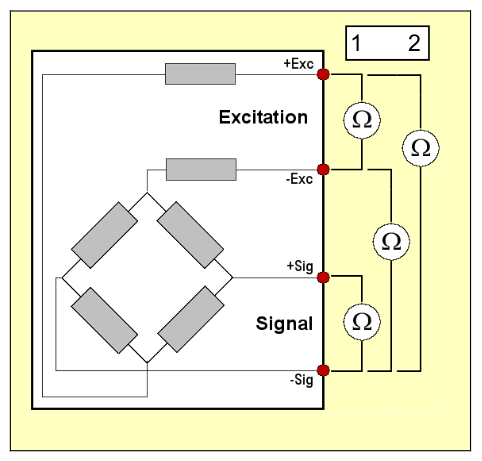
\includegraphics[width=0.4\linewidth]{./images/capteur-force-verif-wheatstone.png}
\end{figure}

\subsection{Sur le site du constructeur}
\subsubsection{Comment peut-on choisir son capteur sur un axe dynamométrique ?}
\paragraph{}
Les capteurs de force sur un axe dynamométrique se trouvent ici :\\
\url{https://fr.scaime.com/axes-dynamometriques-force}.

\paragraph{}
Les capteurs peuvent être choisis en fonction de leur catégorie (mesure de force ou pesage), leur capacité de pesage ($<$50kg, 50kg-500kg, 500kg-5t, 5t-100t), leur charge nominale (0,5 à 2 kN, 1 à 5 kN, ..., jusqu'à 500 à 1 000 kN), leur indice de protection (IP65, IP66, IP67, IP68), leur signal de sortie (4/20mA, 0/10V, mV/V).

\subsubsection{Donner la signification de IP65, IP67, IP68 ?}
\paragraph{}
L'indice de protection est une norme d'étanchéité (EN 60529) qui s'écrit IPxx (pour Indice de Protection suivi de deux chiffres). Le premier chiffre représente l'étanchéité aux corps solides (de 0, aucune protection, à 6, protection contre les poussières) et le second l'étanchéité aux corps liquides (de 0, aucune protection, à 8, protection contre l'immersion pendant une heure et au-delà d'un mètre).

\begin{itemize}
    \item IP65 = protégé totalement contre les poussières et contre les jets d'eau dans toutes les directions.
    \item IP67 = protégé totalement contre les poussières et contre les effets d'une immersion à moins d'un mètre.
    \item IP68 = protégé totalement contre les poussières et contre les effets d'une immersion à plus d'un mètre et dans des conditions spécifiques.
\end{itemize}

\subsubsection{Expliquer les données de la figure suivante : capteur de pesage DVX-D}
\begin{figure}[H]
    \centering
    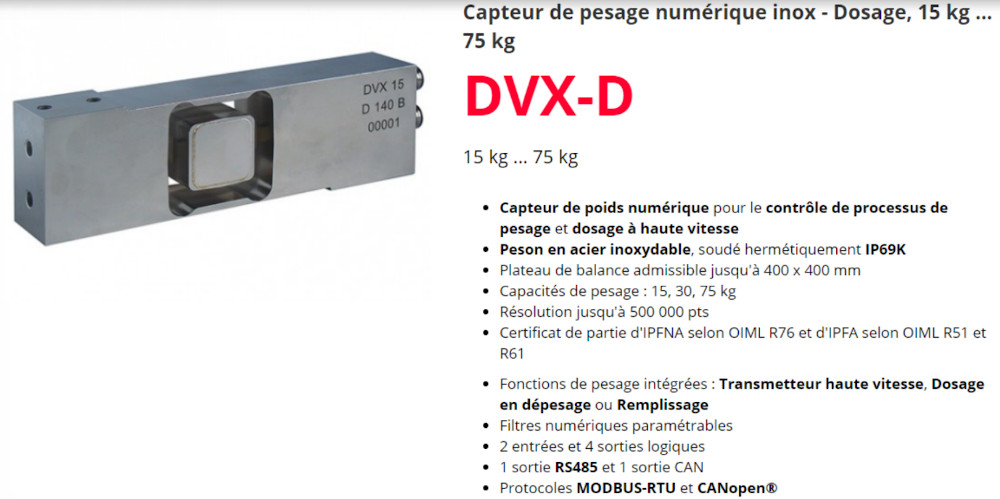
\includegraphics[width=\linewidth]{./images/capteur-force-scaime.jpg}
\end{figure}
\begin{description}
    \item[Capteur de pesage numérique inox - Dosage, 15kg ... 75kg] Il s'agit d'un capteur de pesage qui peut peser jusqu'à 15, 30 ou 75kg en fonction du modèle. Il est utilisé pour le dosage. Ce capteur renvoie un signal numérique.
    \item[Capteur de poids numérique pour le contrôle de processus de pesage et dosage à haute vitesse] C'est le domaine d'application du capteur.
    \item[Peson en acier inoxydable, soudé hermétiquement IP69K] Le capteur est totalement étanche aux poussières et aux liquides. L'IP69K est un indice de protection spécial créé par la norme allemande DIN 40050-9 (puis repris par la norme ISO 20653) pour les équipements qui nécessitent un nettoyage fréquent et intensif : le respect de cette norme garantit l'étanchéité du capteur aux nettoyages à haute pression et à la vapeur.
    \item[Plateau de balance admissible jusqu'à 400 x 400 mm] Il est possible d'utiliser un plateau de balance jusqu'à 40 sur 40cm (à prendre en compte selon la taille de ce qui doit être pesé).
    \item[Capacités de pesage : 15, 30, 75 kg] Selon le modèle, ce capteur peut peser jusqu'à 15, 30 ou 75kg.
    \item[Résolution jusqu'à 500 000 pts] La résolution indique la plus petite variation de mesure détectable par le capteur. Par exempl, pour la capteur allant jusqu'à 75kg, cette résolution sera de $\frac{75}{500000} = 150\si{\micro\gram}$.
    \item[Certificat de partie d'IPFNA selon OIML R76 et d'IPFA selon OIML R51 et R61]\ Il s'agit de normes de l'OIML (Organisation Internationale de Métrologie Légale) concernant les appareils IPFNA (instruments de pesage à fonctionnement non automatique) et IPFA (instrument de pesage à fonctionnement automatique).
    \item[Fonctions de pesage intégrées : Transmetteur haute vitesse, Dosage en dépesage ou remplissage]\ Ce capteur numérique intègre des fonctions qui permettent la mesure en dépesage ou en remplissage ainsi qu'une transmission à haute vitesse (ce qui permet de l'utiliser pour le dosage à haute vitesse).
    \item[Filtres numériques paramétrables] Le capteur contient des filtres dont il est possible de modifier les fréquences filtrées.
    \item[2 entrées et 4 sorties logiques] Ou entrées/sorties TOR.
    \item[1 sortie RS485 et 1 sortie CAN] La norme RS485 (ou EIA-485) définit un mode de communication utilisé en industrie qui permet une communication de type liaison série avec un maximum de 32 appareils, sur une distance allant jusqu'au kilomètre selon la vitesse de transmission. La sortie CAN transmet un signal numérique (convertisseur analogique/numérique).
    \item[Protocoles MODBUS-RTU et CANopen]\ Le protocole MODBUS-RTU fonctionne avec les normes RS232, RS422 et RS485 : c'est un protocole qui fonctionne sur le mode maître-esclave où seul le maître est actif et lit et écrit dans chaque esclave. Le protocole CANopen est un protocole de communication en temps réel où un élément maître du réseau coordonne les éléments esclaves. C'est un protocole très rapide qui peut atteindre 1 Mbit/s.
\end{description}

\newpage
\section{Convertisseur flash (17 février 2020)}
\paragraph{}
Pour le CAN ci-dessous, on demande de :
\begin{enumerate}
    \item Expliquer le fonctionnement du circuit (TV) $Q0$, $Q1$
    \item Donner le mot binaire de sortie $Q_1Q_0$ si $V_{in} = \SI{7}{\volt}$ et $V_{ref} = \SI{10}{\volt}$
\end{enumerate}
\begin{figure}[H]
    \centering
    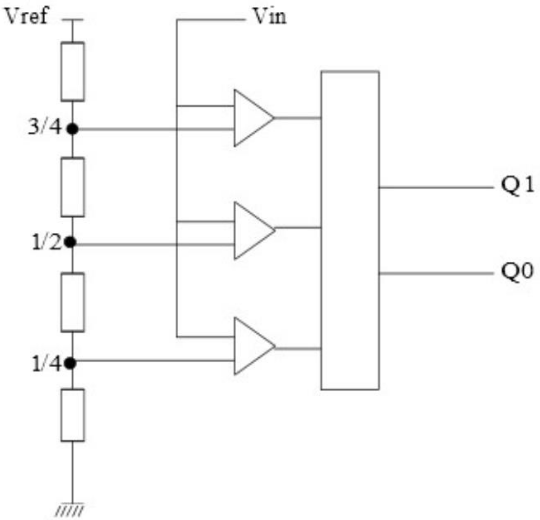
\includegraphics[width=.5\linewidth]{images/convertisseur-flash.png}
\end{figure}

\subsection{Fonctionnement du circuit}
\paragraph{}
Ce circuit permet de transformer un signal analogique ($V_{in}$) en signal numérique codé sur deux bits ($Q_0$ et $Q_1$). Les trois AOP fonctionnent en comparateur entre $V_{in}$ et $V_{ref}$ divisée par un pont diviseur :
\begin{itemize}
    \item Pour $V_{in}$ entre 0 et $\frac{1}{4} V_{ref}$ : $Q_1Q_0 = 00$
    \item Pour $V_{in}$ entre $\frac{1}{4} V_{ref}$ et $\frac{1}{2} V_{ref}$ : $Q_1Q_0 = 01$
    \item Pour $V_{in}$ entre $\frac{1}{2} V_{ref}$ et $\frac{3}{4} V_{ref}$ : $Q_1Q_0 = 10$
    \item Pour $V_{in}$ supérieur à $\frac{3}{4} V_{ref}$ : $Q_1Q_0 = 11$
\end{itemize}

\subsection{Mot binaire de sortie $Q_1Q_0$}
\paragraph{}
si $V_{in} = \SI{7}{\volt}$ et $V_{ref} = \SI{10}{\volt}$

\paragraph{}
$\frac{1}{2} V_{ref} < V_{in} < \frac{3}{4} V_{ref} \Rightarrow Q_1Q_0 = 10$


\newpage
\section{CNA à résistances pondérées (17 février 2020)}
\paragraph{}
Pour le circuit ci-dessous; on demande de
\begin{enumerate}
    \item Déterminer l'équation de la sortie $V_s = f(ai, V_{ref})$
    \item Calculer la tension de sortie si $V_{ref} = \SI{10}{\volt}$
\end{enumerate}
\begin{figure}[H]
    \centering
    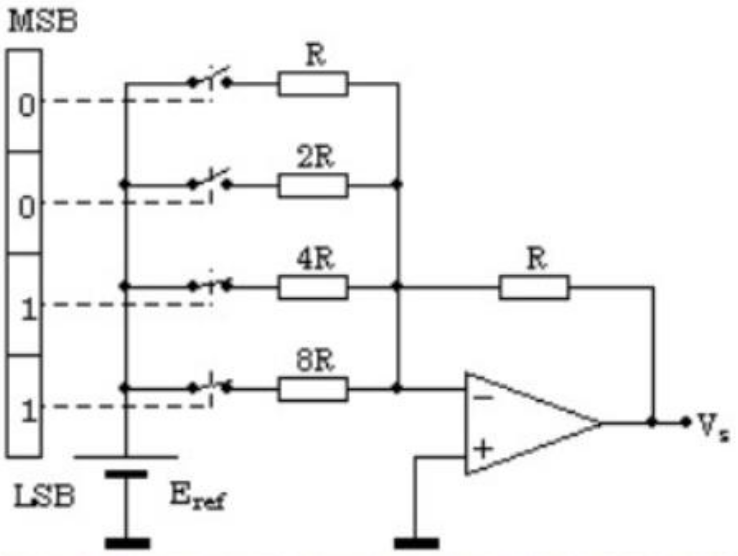
\includegraphics[width=.5\linewidth]{images/CNA-resistances-ponderees.png}
\end{figure}

\subsection{Équation de la tension de sortie}
\paragraph{}
L'AOP est monté en sommateur inverseur :
\begin{align*}
    V_s &= -R \left(\frac{V_{ref}D_0}{8R} + \frac{V_{ref}D_1}{4R} + \frac{V_{ref}D_2}{2R} + \frac{V_{ref}D_3}{R} + \right)\\
    V_s &= -\frac{V_{ref}}{8} \left(D_0 + 2D_1 + 4D_2 + 8D_3\right)\\
\end{align*}

\subsection{Calcul de la tension de sortie}
\paragraph{}
avec $V_{ref} = \SI{10}{\volt}$, $D_0 = 1$, $D_1 = 1$, $D_2 = 0$ et  $D_3 = 0$.
\begin{align*}
    V_s &= -\frac{10}{8} \left(1 + 2\right)\\
    V_s &= -3,75 \si{\volt}\\
\end{align*}


\newpage
\section{Datasheet D-Z76 (2 mars 2020)}
\paragraph{}
Trouver la datasheet du composant D-Z76 et répondre aux questions suivantes :
\begin{enumerate}
    \item Quelles sont ses caractéristiques ?
    \item Peut-on inverser la polarité du capteur ?
    \item Est-il compatible avec les PLC ?
    \item Donner la constitution interne de ce type de capteur et expliquer son fonctionnement
    \item Traduire les termes suivants : lead wire, leakage current, heavy duty, enclosure, insulation resistance, withstand voltage between lead wire and case, internal voltage drop, reed switch, red, brown, blue, black.
    \item Où peut on trouver ce capteur dans une ligne de production ?
    \item Comment pouvez vous tester le bon fonctionnement de ce capteur sur site?
    \item Hors site ?
    \item Comparez le D-Z76 avec le D-Z73
\end{enumerate}

\subsection{Caractéristiques du D-Z76}
\begin{figure}[H]
    \centering
    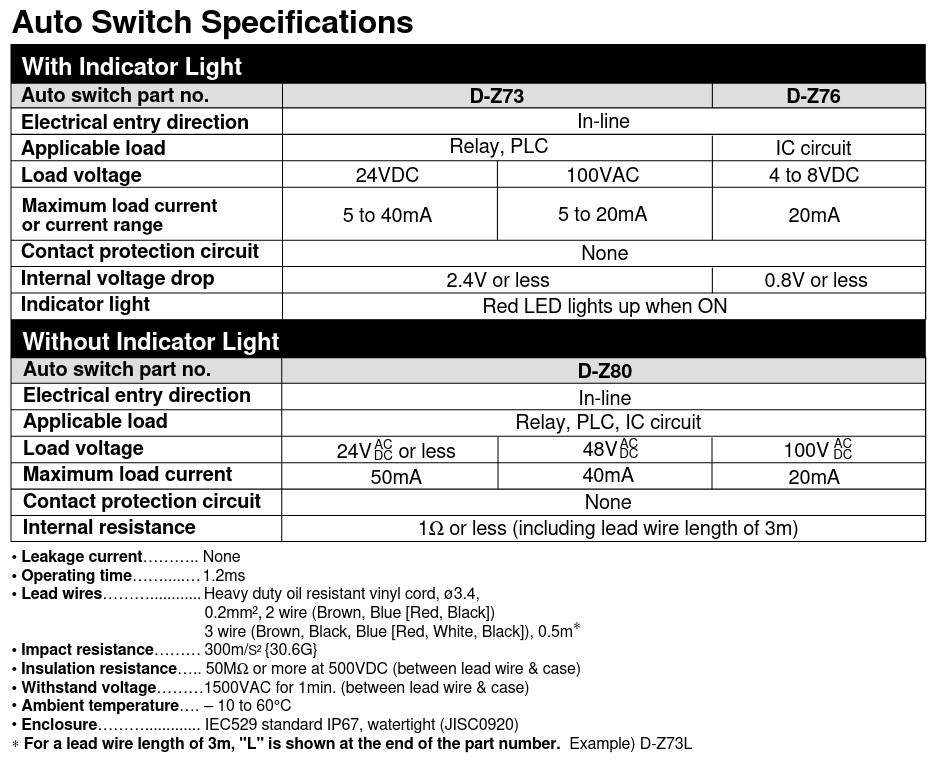
\includegraphics[width=.8\linewidth]{images/D-Z76-specs.png}
\end{figure}

\begin{table}[H]
    \begin{center}
        \begin{tabular}{l l}
            \textbf{Application} & intégration dans un circuit CI\\
            \hline
            \textbf{Tension de charge} & 8 V DC\\
            \hline
            \textbf{Courant de charge max} & 20 mA\\
            \hline
            \textbf{Circuit de protection} & aucun\\
            \hline
            \textbf{Chute de tension interne} & max 0.8 V\\
            \hline
            \textbf{Indicateur lumineux} & LED rouge (allumée quand le switch est ON)\\
            \hline
            \textbf{Courant de fuite} & aucun\\
            \hline
            \textbf{Temps de réponse} & 1.2 ms\\
            \hline
            \textbf{Câbles de connexion} & Hautement résistants \diameter 3.4, 0.2 $\si{\milli\meter^2}$, \\
            & 3 fils (brun/noir/bleu [rouge/blanc/noir]), 0.5m\\
            \hline
            \textbf{Résistance aux chocs} & 300 \si{\meter}/S$^2$ (30.6G)\\
            \hline
            \textbf{Résistance d'isolement} & 50\si{\mega\ohm} ou plus à 500 VDC (entre les connections et le boitier)\\
            \hline
            \textbf{Tension nominale} & 1500 VAC pendant 1 min (entre les connections et le boitier)\\
            \hline
            \textbf{Température de fonctionnement} & entre -10 et 60\si{\celsius}\\
            \hline
            \textbf{Protection} & IP67 (IEC529), étanche (JISC0920)\\
        \end{tabular}
    \end{center}
\end{table}

\subsection{Peut-on inverser la polarité du capteur ?}
\paragraph{}
Non, il n'y a aucun circuit de protection.

\subsection{Est-il compatible avec les PLC ?}
\paragraph{}
Non, seuls les modèles D-Z73 et D-Z80 sont compatibles avec les PLC (programmable logic controller, automate programmable industriel).

\subsection{Donner la constitution interne de ce type de capteur et expliquer son fonctionnement}

\begin{figure}[H]
    \centering
    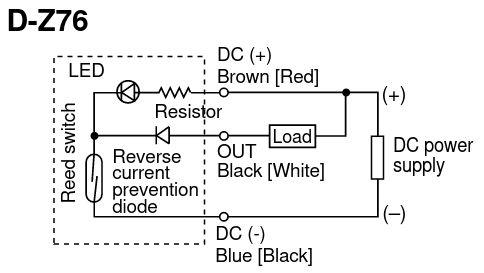
\includegraphics[width=.5\linewidth]{images/D-Z76-schema.png}
\end{figure}

\paragraph{}
Ce détecteur se base sur l'effet magnétique : un interrupteur reed NO qui se ferme en présence d'un champs magnétique. L'interrupteur Reed ou ILS (interrupteur à lames souples) est généralement constitué d'une ampoule de verre protectrice contenant une atmosphère non oxydante et deux contacts souples magnétisables et élastiques. En présence d'un champ magnétique, les contacts s'aimantent par influence, et sont attirés l'un par l'autre. Ils se rapprochent et se touchent, établissant le courant. Lorsque le champ magnétique cesse, l'aimantation cesse aussi, et l'élasticité des contacts les écarte, coupant le courant. (source : \href{https://fr.wikipedia.org/wiki/Interrupteur_reed}{Wikipédia})


\paragraph{}
Le détecteur est alimenté en courant continu par les fils brun [rouge] (+) et bleu [noir] (-). La charge doit être connectée entre les fils brun [rouge] et noir [blanc].

\paragraph{}
Le détecteur est équipé d'une LED qui indique sont fonctionnement (quand le switch est fermé, la LED s'allume). Une diode le protège des inversions de courant.

\subsection{Traduction des termes techniques}
\begin{table}[H]
    \begin{center}
        \begin{tabular}{l l}
            \textbf{lead wire} & fil de connection \\
            \textbf{leakage current} & courant de fuite \\
            \textbf{heavy duty} & très résistant \\
            \textbf{enclosure} & boîtier \\
            \textbf{insulation resistance} & résistance d'isolement\\
            \textbf{withstand voltage} & tension nominale\\
            \textbf{between lead wire and case} & entre les connexions et le boîtier\\
            \textbf{internal voltage drop} & chute de tension interne\\
            \textbf{reed switch} & switch (commutateur) Reed\\
            \textbf{red, brown, blue, black} & rouge, brun, bleu, noir\\
        \end{tabular}
    \end{center}
\end{table}

\subsection{Où peut on trouver ce capteur dans une ligne de production ?}
\paragraph{}
Capteurs de fin de course pour les vérins, générateur d'impulsion de comptage, etc.

\subsection{Comment pouvez vous tester le bon fonctionnement de ce capteur sur site?}
\paragraph{}
Grâce à la LED qui indique le fonctionnement du capteur.

\subsection{Hors site ?}
Dans le capteur tel qu'il est, rien ne permet de vérifier son bon fonctionnement sans au minimum un contact visuel.

\subsection{Comparez le D-Z76 avec le D-Z73}
\paragraph{}
Les deux détecteurs se distinguent sur les caractéristiques suivantes :

\begin{table}[H]
    \begin{center}
        \begin{tabular}{c c c}
            & \textbf{D-Z73} & \textbf{D-Z76} \\
            \hline
            \textbf{Application} & relais, API & circuit CI \\
            \hline
            \textbf{Tension de charge} & 24VDC / 100VAC & 8VDC\\
            \hline
            \textbf{Courant de charge max} & 5 à 40mA / 5 à 20mA & 20mA\\
            \hline
            \textbf{Chute de tension interne} & max 2.4V & max 0.8V\\
            \hline
            \textbf{Temps de réponse} & 1.2 ms\\
            \hline
            \textbf{Câbles de connexion} & 2 câbles (brun/bleu [rouge/noir]) & 3 câbles (brun/noir/bleu)\\
             &  & [rouge/blanc/noir])\\
        \end{tabular}
    \end{center}
\end{table}

\newpage
\paragraph{}
Circuits internes :
\begin{figure}[H]
    \centering
    \begin{subfigure}{.4\textwidth}
        \centering
        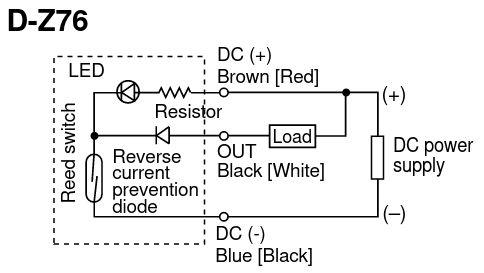
\includegraphics[width=\linewidth]{./images/D-Z76-schema.png}
    \end{subfigure}
    \begin{subfigure}{.4\textwidth}
        \centering
        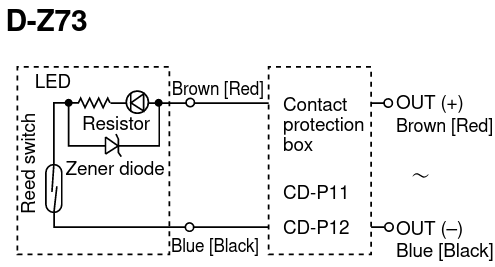
\includegraphics[width=\linewidth]{./images/D-Z73-schema.png}
    \end{subfigure}
\end{figure}


\newpage
\section{Labo 1 : Interface à LED (2 mars 2020)}
\paragraph{}
Pour le schéma suivant :
\begin{enumerate}
    \item Choisir la résistance R (valeur, $P_{max}$ et tolérance)
    \item Vérifier au multimètre R, I et U
\end{enumerate}

\begin{figure}[H]
    \centering
    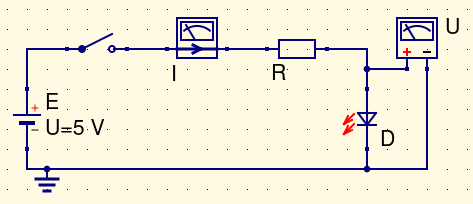
\includegraphics[width=.6\linewidth]{images/labo1.png}
\end{figure}

\subsection{Choix de la résistance}
\paragraph{Valeur de R :}
\begin{description}
    \item[$U_{LED}$] $= 2\si{\volt}$ (entre $1,8\si{\volt}$ et $2,2\si{\volt}$)
    \item[$I_{LED}$] $= 20\si{\milli\ampere}$ (conseillé entre $16\si{\milli\ampere}$ et $18\si{\milli\ampere}$)
    \item[$U_R$] $= U - U_{LED} = 3\si{\volt}$
    \item[$R$] $= \frac{U}{I} = \frac{3}{17.10^{-3}} = 176,471\si{\ohm}$
\end{description}
La valeur normalisée de résistance s'en rapprochant le plus est \SI{180}{\ohm} ($I = 16,667\si{\milli\ampere}$)

\paragraph{Puissance de R :}
\begin{description}
    \item[$P_{max}$] $= U.I = 3.16,667.10^{-3} = 50 \si{\milli\watt}$)
\end{description}
On peut prendre n'importe quelle puissance de résistance, le minimum étant 1/8\si{\watt} (ici j'utilise une résistance de 1/4\si{\watt}).

\paragraph{Tolérance de R :}
\begin{description}
    \item[$R_{max}$] $= \frac{U_{max}}{I} = \frac{3,2}{16,667.10^{-3}} = 192 \si{\ohm}$)
    \item[$R_{min}$] $= \frac{U_{min}}{I} = \frac{2,8}{16,667.10^{-3}} = 168 \si{\ohm}$)
\end{description}

\paragraph{}
Pour la résistance choisie de 180\si{\ohm} :
\begin{description}
    \item[Tolérance max] = $\frac{100(192 - 180)}{180} = 6,667\%$ 
    \item[Tolérance min] = $\frac{100(180 - 168)}{180} = 6,667\%$ 
\end{description}
Une tolérance de $\pm5\%$ (ou moins) convient pour ce montage.

\subsection{Vérification au multimètre}
\paragraph{Montage réalisé :}\
\begin{figure}[H]
    \centering
    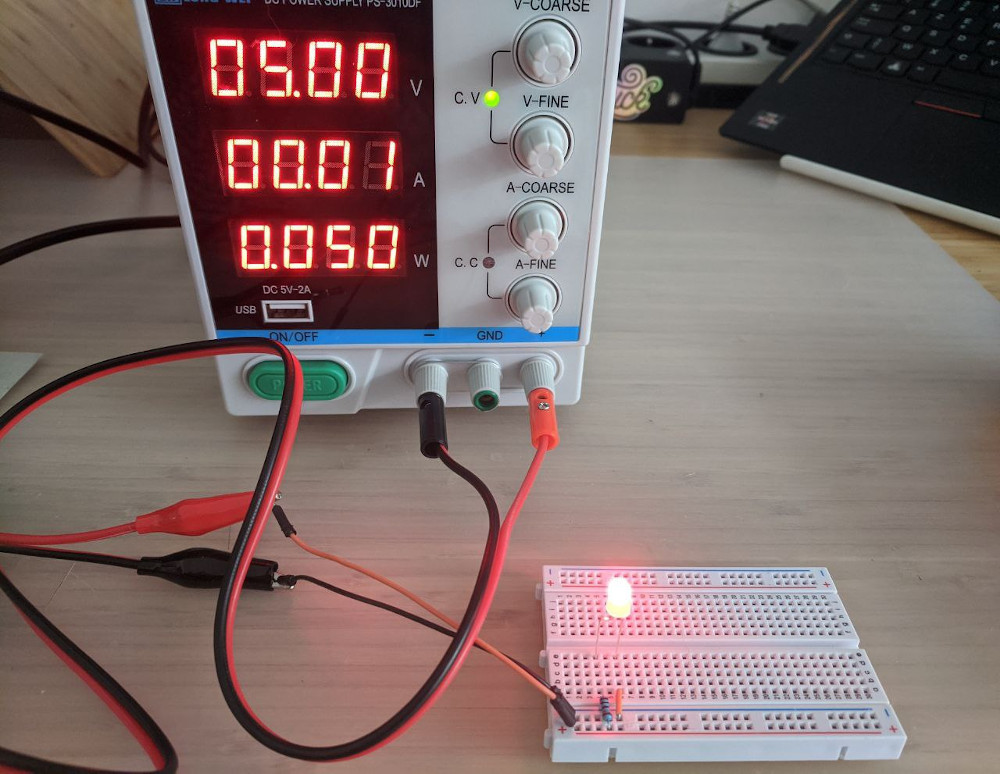
\includegraphics[width=.6\linewidth]{images/labo1-montage.jpg}
\end{figure}

\paragraph{Valeurs mesurées :}
\begin{description}
    \item[$U_{LED}$] = $1,959 \si{\volt}$ 
    \item[$U_{R}$] = $2,915 \si{\volt}$ 
    \item[$I$] = $16,09 \si{\milli\ampere}$ (voir image suivante)
\end{description}

\begin{figure}[H]
    \centering
    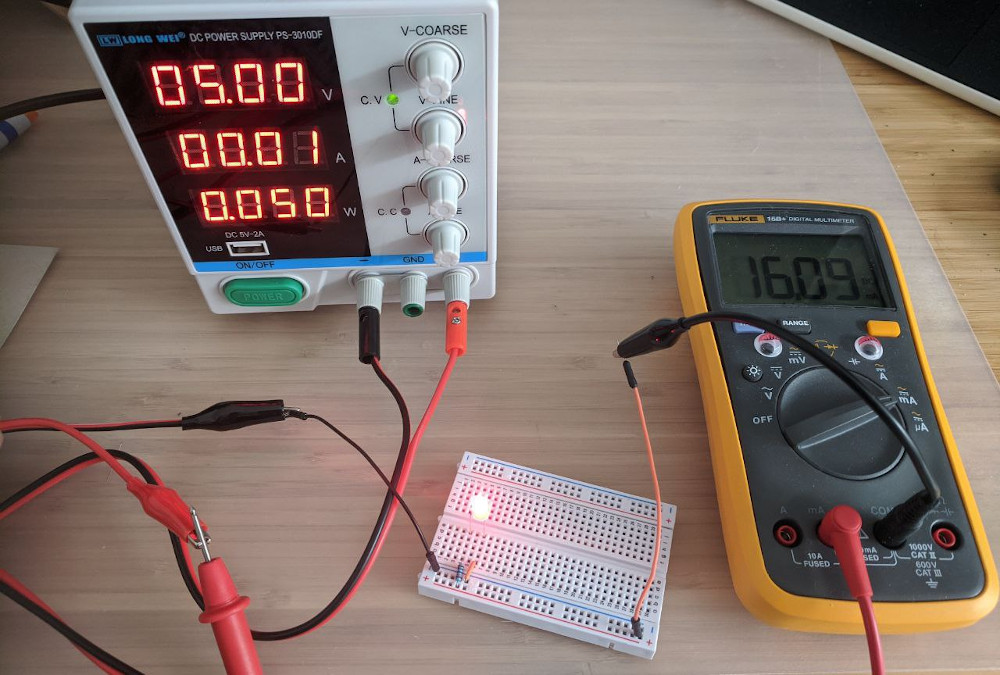
\includegraphics[width=.6\linewidth]{images/labo1-courant.jpg}
\end{figure}

\subsection{Vérification avec Qucs}
\begin{figure}[H]
    \centering
    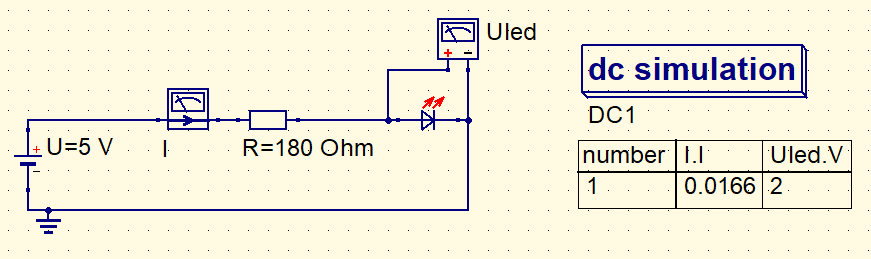
\includegraphics[width=.8\linewidth]{images/labo1-qucs.png}
\end{figure}


\newpage
\section{Labo 2 : Interface transistor NPN (9 mars 2020)}
\paragraph{}
Pour le schéma suivant :
\begin{enumerate}
    \item Rechercher sur internet labo2 datasheet du BC547B
    \item Déterminer $V_{bb}$, $I_b$, $R_1$ et $R_2$ si $V_{cc} = \SI{5}{\volt}$
    \item Réaliser le montage et mesurer $I_c$, $I_b$ , $U_{LED}$ et $U_{be}$
\end{enumerate}
\begin{figure}[H]
    \centering
    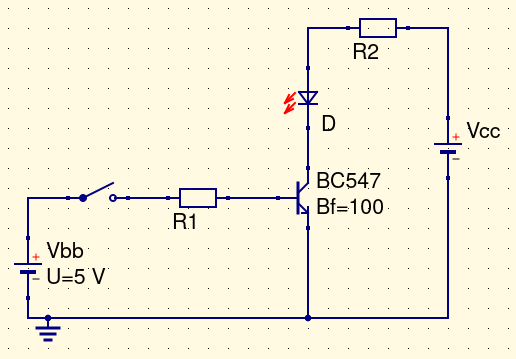
\includegraphics[width=.6\linewidth]{images/labo2.png}
\end{figure}

\subsection{Datasheet du transistor BC547B}
\paragraph{}
Liens :
\begin{description}
    \item \url{https://www.farnell.com/datasheets/410427.pdf}
    \item \url{https://diotec.com/tl_files/diotec/files/pdf/datasheets/bc546.pdf}
\end{description}

\begin{description}
    \item[$V_{CE max}$] = $45 \si{\volt}$ 
    \item[$I_{C max}$] = $100 \si{\milli\ampere}$
    \item[$P_{max}$] = $500 \si{\milli\watt}$ %≃Vce.Ic (+Vbe.Ib)-> négligeable
    \item[$h_{FE}$] = 200 %= IC/IB => pas d'unité 
    \item[$V_{CE sat}$] = 0,25\si{\volt}
    \item[$V_{BE}$] = 0,7\si{\volt}
\end{description}

\paragraph{NB}
Pour $V_{CE} = \SI{5}{\volt}$ et $I_C = \SI{2}{\milli\ampere}$ :
\begin{description}
    \item[$h_{FE}$ $A$] = entre 110 et 220
    \item[$h_{FE}$ $B$] = entre 200 et 450
    \item[$h_{FE}$ $C$] = entre 420 et 800
\end{description}
% on prend toujours la valeur min pour être sûr qu'ils communiquent bien
Ici, on est dans le groupe B : le gain minimum est de 200.


\subsection{Déterminer $V_{cc}$, $I_b$, $R_1$ et $R_2$}
\paragraph{}si $V_{bb} = \SI{5}{\volt}$

\begin{description}
    \item[$V_{cc max}$] = 40V. Ici on utilise $V_{cc} = 5V$
    \item[$I_b$] = $\frac{I_c}{h_{FE}}.2$(pour être sûr de saturer le transistor) $= \frac{20.10^{-3}}{200} = 100\si{\micro\ampere}$ 
    \item[$R_2$] = $\frac{V_{cc} - V_{CE sat} - V_{LED}}{I_{LED}} = \frac{5 - 0,25 - 2}{10.10^{-3}} = 275\si{\ohm} \approx 270\si{\ohm}$ (valeur normalisée)
    \item[$R_1$] = $\frac{V_{bb} - V_{BE}}{I_{b}} = \frac{5 - 0,7}{10^{-4}} = 43\si{\kilo\ohm} \approx 47\si{\kilo\ohm}$ (valeur normalisée)
\end{description}

\subsection{Réaliser le montage et mesurer $I_c$, $I_b$ , $U_{LED}$ et $U_{be}$}
\paragraph{}Valeurs mesurées :
\begin{description}
    \item[$V_{BE}$] = $700\si{\milli\volt}$
    \item[$V_{CE}$] = $50\si{\milli\volt}$
    \item[$I_b$] = $275\si{\micro\ampere}$
    \item[$I_c$] = $6,5\si{\milli\ampere}$
\end{description}

\subsection{Vérification avec Qucs}
\begin{figure}[H]
    \centering
    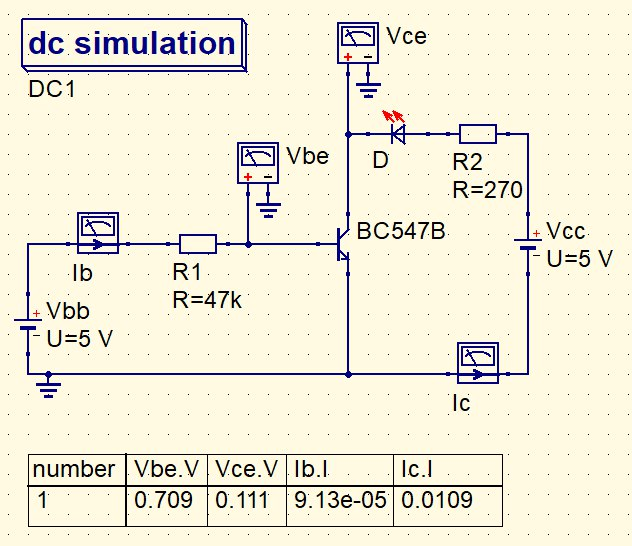
\includegraphics[width=.6\linewidth]{images/labo2-qucs.jpg}
\end{figure}


\newpage
\section{Labo 3 : Montage d’un capteur résistif en TOR (9 mars 2020)}
Pour le schéma suivant :
\begin{enumerate}
    \item Choisir $V_{cc}$, Pot et $R_2$ (outil : datasheet LM393*)
    \item Expliquer le fonctionnement et tracer sa caractéristique de transfert
    \item Câbler et tester le circuit sur breadboard
\end{enumerate}
*Pour refaire ce labo, j'ai utilisé un AOP simple TL071
\begin{figure}[H]
    \centering
    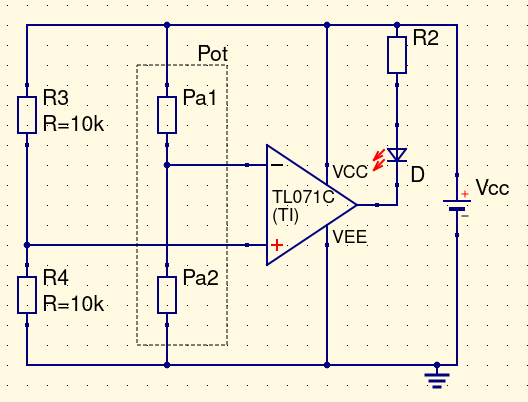
\includegraphics[width=.6\linewidth]{images/labo3.png}
\end{figure}

\subsection{Choix de $V_{cc}$, Pot et $R_2$}
\begin{description}
    \item[$V_{cc}$] = $12\si{\volt}$
    \item[$Pot$] = $10\si{\kilo\ohm}$
    \item[$R_2$] = $\frac{V_{cc} - V_D}{I_D} = \frac{12 - 2}{20.10^{-3}} = 500\si{\ohm} \approx 510 \si{\ohm}$
\end{description}

\subsection{Fonctionnement du circuit}
\paragraph{}
L'AOP fonctionne en comparateur par rapport à une tension de 6V. Si la tension de sortie du potentiomètre (Pa2) est inférieure, la tension de sortie de l'AOP est à $V_{cc}$, il n'y a pas de différence de potentiel aux bornes de la LED qui reste éteinte. Si elle est supérieure à 6V, supérieure, la tension de sortie de l'AOP est à 0V, ce qui crée une différence de potentiel aux bornes de la LED et elle s'allume.
\paragraph{}
Avec le LM393, le circuit ne fonctionne pas en fonctionnement inverse (la LED entre la sortie de l'AOP et la terre) car le circuit de l'AOP se termine avec un transistor qui se retrouve alors connecté à rien. L'avantage de terminer le circuit par un transistor est de pouvoir mettre une autre tension d'alimentation en sortie.

\paragraph{}Caractéristique de transfert :
\begin{figure}[H]
    \centering
    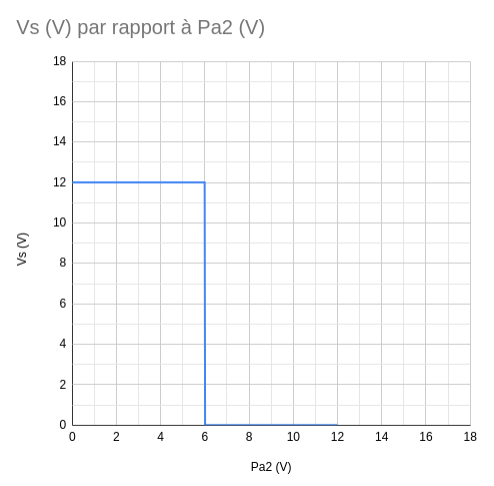
\includegraphics[width=.6\linewidth]{images/labo3-caract-transfert.png}
\end{figure}

\newpage
\subsection{Câbler et tester le circuit}
\paragraph{}Montage réalisé :
\begin{figure}[H]
    \centering
    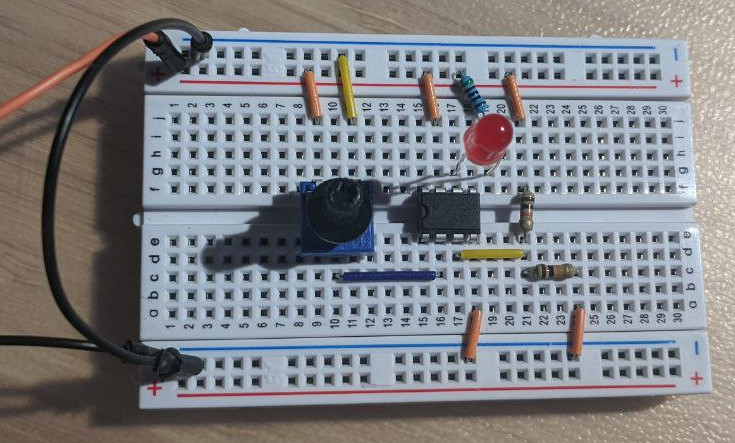
\includegraphics[width=.8\linewidth]{./images/labo3-montage.jpg}
\end{figure}

\paragraph{}Test :
\begin{figure}[H]
    \centering
    \begin{subfigure}{.4\textwidth}
        \centering
        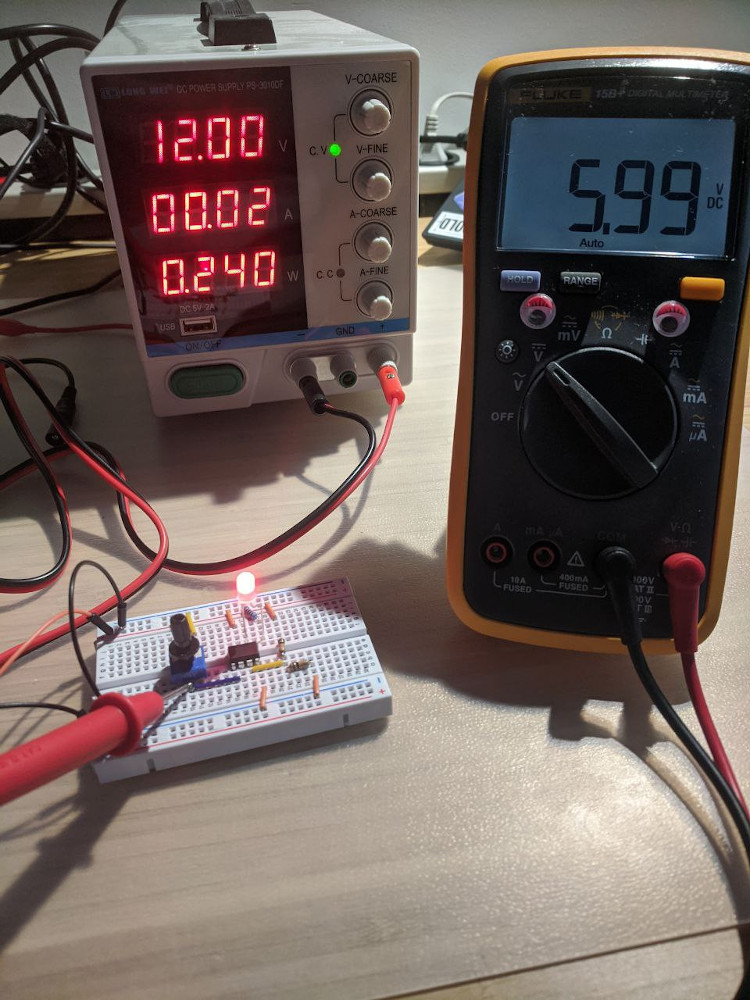
\includegraphics[width=.9\linewidth]{./images/labo3-verif1.jpg}
    \end{subfigure}
    \begin{subfigure}{.4\textwidth}
        \centering
        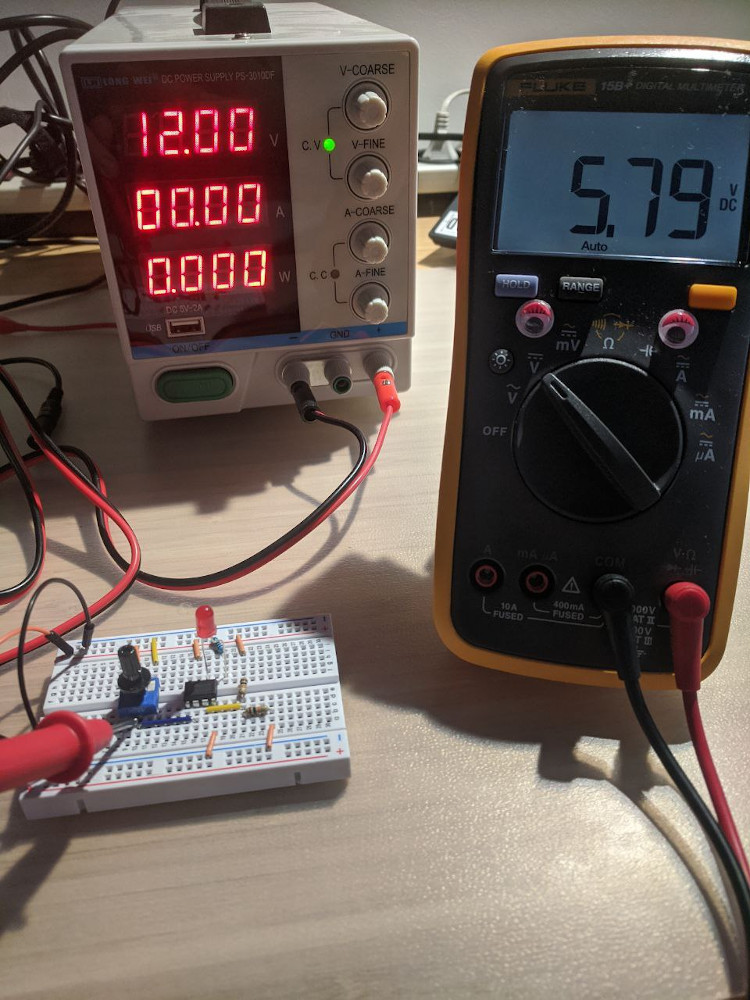
\includegraphics[width=.9\linewidth]{./images/labo3-verif2.jpg}
    \end{subfigure}
\end{figure}
La LED s'allume ou s'éteint lorsque la tension aux bornes du potentiomètre approche les 6V.

\subsection{Vérification avec Qucs}
\paragraph{}Mesure des tensions :
\begin{figure}[H]
    \centering
    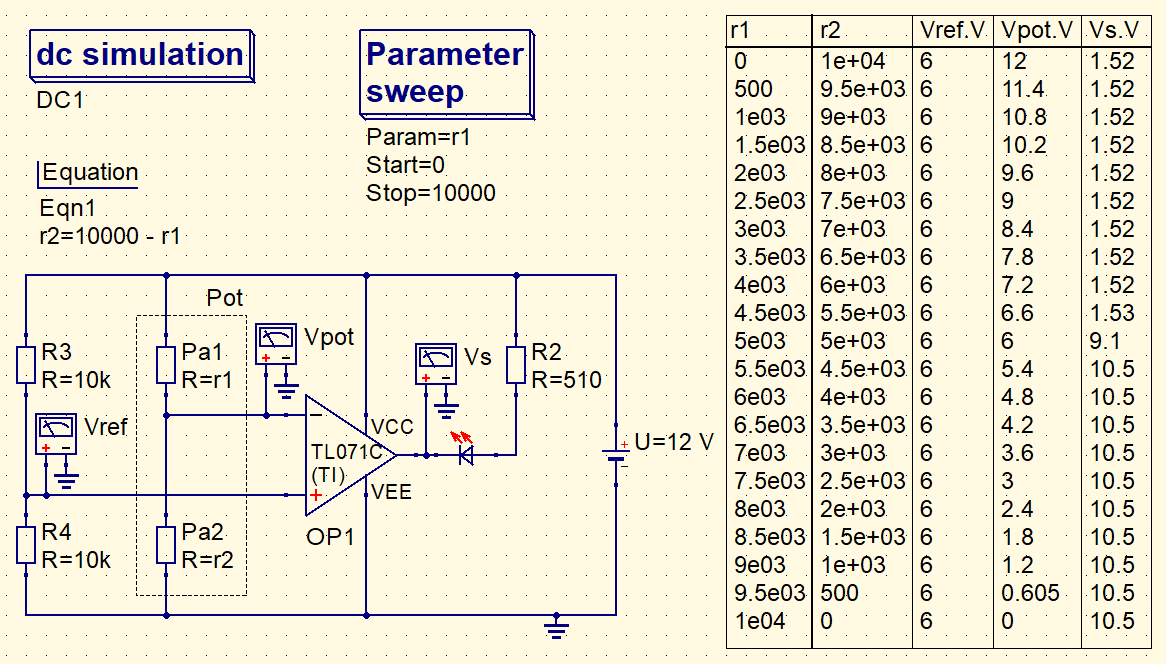
\includegraphics[width=.95\linewidth]{./images/labo3-qucs.png}
\end{figure}

\paragraph{}
Caractéristique de transfert :
\begin{figure}[H]
    \centering
    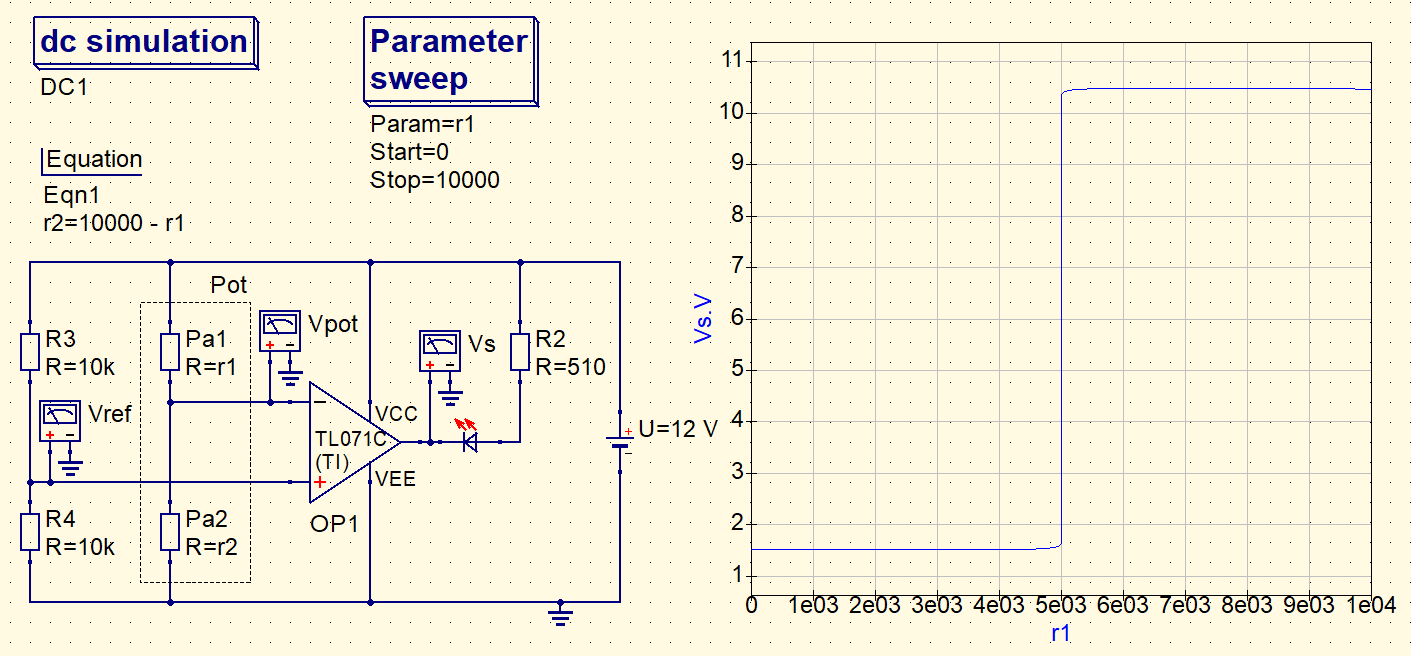
\includegraphics[width=.95\linewidth]{./images/labo3-qucs-caract-transfert.png}
\end{figure}



\newpage
\section{CAN exercice 1 : automate pressostat (23 mars 2020)}
\paragraph{}
Afin d'adapter la vitesse de fonctionnement du moteur à la pression P du réseau de sortie, on mesure la pression à l'aide d'un capteur de pression PT monté sur le réseau de sortie d'eau. Le pressostat fournit ensuite une tension continue $U_{PT}$, image de la pression P.

\begin{figure}[H]
    \centering
    \includegraphics[width=.6\linewidth]{images/acq-ex1-enonce.jpg}
\end{figure}

\paragraph{}
Le convertisseur analogique-numérique utilisé sera considéré comme ayant une résistance d'entrée infinie d'où i=0. Pour le pressostat $U_{PT} = kP$ avec $k = 2,0\si{\volt\per\bar}$; la pression maximale à mesurer est de 10\si{\bar}.

\paragraph{}
On donne :
\begin{itemize}
    \item $R_2 = \SI{1}{\kilo\ohm}$ et le curseur du potentiomètre est en position médiane.
    \item $R_3 = \SI{1}{\kilo\ohm}$.
\end{itemize}

\paragraph{}
\begin{enumerate}
    \item Calculer la valeur à donner à la résistance $R_1$, sachant que la tension $u_0$ appliquée à la carte contrôle du variateur doit être égale à 10V lorsque la pression à mesurer est maximale.
    \item Le convertisseur analogique-numérique doit pouvoir convertir une tension $u_0$ comprise entre 0 et $U_{0max} = 10\si{\volt}$; la tension $u_0$ est codée sur n = 8 bits; on définit la résolution r = $U_{0max}$/$2^n$. Calculer r et en déduire la plus petite valeur de la pression que l'on peut mesurer.
    \item La pression P sur le réseau de sortie d'eau est fixé à 6\si{\bar}. Quel sera le mot binaire qui codera la tension $u_0$ correspondante ?
\end{enumerate}

\subsection{Calculer la valeur de $R_1$}
\paragraph{}
sachant que $u_0$ = 10V lorsque la pression à mesurer est maximale.

\begin{description}
    \item[$U_{PTmax}$] = $f.P_{max} = 2.10 = 20 \si{\volt}$ 
\end{description}

\paragraph{}
Puisque $u_{0max}$ = 10V, il faut diviser la tension $U_{PT}$ par 2 :
\begin{align*}
    R_1 + \frac{R_2}{2} &= \frac{R_2}{2} + R_3\\
    R_1 &= R_3 = \SI{1}{\kilo\ohm}
\end{align*}

\subsection{Calculer r et en déduire la plus petite valeur de la pression que l'on peut mesurer}
\paragraph{}
sachant que $0 < u_0 < 10$V, que $u_0$ est codée sur n = 8 bits et que la résolution r = $U_{0max}$/$2^n$.

$$r = \frac{U_{0max}}{2^n - 1} = \frac{10}{2^8 - 1} = 39,216\si{\milli\volt}$$
\paragraph{}
Puisque la tension $U_{0max} = 10\si{\volt}$ correspond à une pression mesurée $P_{max} = 10\si{\bar}$, dispositif de mesure avance par pas de 39,216\si{\milli\bar}.

\subsection{Quel sera le mot binaire qui codera la tension $u_0$ correspondant à une pression P de 6\si{\bar} ?}
$$\frac{P}{r} = \frac{6}{39,216.10^{-3}} = 153_{dec} = 1001\,1001_{bin} = 99_{hex}$$


\newpage
\section{CAN exercice 2 : masse d'une essoreuse (23 mars 2020)}
\paragraph{}
La masse d'une essoreuse est mesurée par un système de pesage analogique délivrant un signal 4-20\si{\milli\ampere} pour une masse variant de 0 à 4000\si{\kilogram}. La conversion est effectuée par un convertisseur 14bits en code binaire naturel.

\begin{enumerate}
    \item donner la résolution (en masse) du convertisseur
    \item à quelle combinaison en hexadécimal correspond une masse de 400kg?
    \item à quel courant correspond cette masse ?
\end{enumerate}

\subsection{Résolution du convertisseur}
$$r = \frac{m_{max} - m_{min}}{2^{nbits} - 1} = \frac{4000 - 0}{2^{14} - 1} = 244,156\si{\gram}$$

\subsection{Mot hexadécimal correspondant à une masse de 400kg}
400kg correspond à $\frac{400}{4000}\left(2^{14} - 1\right) = 1638_{dec} = 110 0110 0110_{bin} = 666_{hex}$

\subsection{Courant correspondant à une masse de 400kg}
$$I_{400} = m\frac{(I_{max} - I_{min})}{m_{max} - m_{min}} + offset = 400\frac{(20-4).10^{-3}}{4000 - 0} + 4.10^{-3} = 5,6\si{\milli\ampere}$$

\paragraph{}
L'équation pour trouver le courant de sortie en fonction de la masse pesée est :
\begin{align*}
    i &= m\frac{(20 - 4).10^{-3}}{4000} + 4.10^{-3}\\
    i &= 4m.10^{-6} + 4.10^{-3}
\end{align*}

\paragraph{}
Caractéristique de transfert :
\begin{figure}[H]
    \centering
    \includegraphics[width=.6\linewidth]{./images/CAN-ex2-caract-transfert.png}
\end{figure}


\newpage
\section{Choix d'une carte d'acquisition et de restitution des données (23 mars 2020)}
%(Traitement des signaux et acquisition de données, Francis Cottet, Dunod)

\paragraph{}
On considère une application industrielle à instrumenter. Cette application est caractérisée par ses entrées/ sorties au niveau des capteurs et des actionneurs utilisés. Soit :
\begin{itemize}
    \item 2 actionneurs tout ou rien avec un temps de réponse de 20ms
    \item un actionneur à commande spécifié par :
    \begin{itemize}
        \item fréquence maximale de restitution : 3kHz
        \item variation de la tension à fourni : de -5V à +5V
        \item précision de la tension de commande : 5mV
    \end{itemize}
    \item un premier capteur spécifié par :
    \begin{itemize}
        \item fréquence maximale d'acquisition : 100Hz
        \item variation de la tension fournie par le capteur : 0 à 10mV
        \item précision de mesure : 10\si{\micro\volt}
    \end{itemize}
    \item un deuxième capteur spécifié par :
    \begin{itemize}
        \item fréquence maximale d'acquisition : 10kHz
        \item variation de la tension fournie par le capteur : 0 à 1V
        \item précision de mesure : 5mV
    \end{itemize}
\end{itemize}

\paragraph{}
Choisir la carte la plus adaptée à cette application parmi les suivantes :
\begin{figure}[H]
    \centering
    \includegraphics[width=.75\linewidth]{images/choix-carte.jpg}
\end{figure}

\paragraph{Réponse}
\paragraph{}
La carte B est la seule à répondre à tous les critères.

\paragraph{}
La carte A est éliminée car elle n'a pas d'entrée TOR alors qu'il en faut 2 (en pratique, les entrées analogiques peuvent être utilisées en TOR et la carte A pourrait aussi être gardée).

\paragraph{}
La carte E est éliminée car ses sorties analogiques ne permettent pas de fournir une tension allant de -5V à 5V : sa tension de sortie est de 0 à 10V alors que l'actionneur a besoin d'une tension entre -5 et 5V.

\paragraph{}
La carte D est éliminée car il faudrait un gain de $10^3$ pour passer des 0 à 10mV fournis par le capteur 1 aux 0 à 10V en entrée de la carte. Or, le gain programmable de la carte ne va que jusque $10^2$.

\paragraph{}
La carte C est éliminée car elle n'offre pas une résolution suffisante pour le capteur 1. Le capteur 1 fournit un signal de 0 à 10mV et sa précision doit être de 10\si{\micro\volt} : son nombre de pas minimum doit être de $\frac{(10-0).10^{-3}}{10.10^{-6}} + 1 = 1001$. Sa résolution minimale devrait être de 10bits ($2^{10} = 1024$ valeurs). Or, la carte C n'offre qu'une résolution de 8bits.


\newpage
\section{Labo 4 : Commande d'un four (30 mars 2020)}
\paragraph{}
On désire visualiser à l'aide de deux LEDs la température d'un four par rapport à deux températures limites $\Theta_a = \SI{180}{\celsius}$ et $\Theta_b = \SI{200}{\celsius}$. La température du four est captée par une résistance à coefficient de température négatif : $R = \SI{30}{\kilo\ohm}$ à $\SI{180}{\celsius}$ et $R = \SI{10}{\kilo\ohm}$ à $\SI{200}{\celsius}$.

\begin{figure}[H]
    \centering
    \includegraphics[width=.8\linewidth]{images/four.png}
\end{figure}

\paragraph{}
Déterminer les valeurs de
\begin{enumerate}
    \item $V_a$, $V_b$ et $V$ pour $\Theta_a$ et $\Theta_b$
    \item $R_2$ et $R_3$ pour obtenir $V_1 = V_b$ et $V_2 = V_a$
    \item Déterminer quand les LEDs sont allumées et éteintes
    \item Tracer la caractéristique de transfert de la CTN
    \item Tracer le schéma adapté sous Qucs
    \item Réaliser et tester le montage sur breadboard en ajoutant la carte relais sur une des sorties
\end{enumerate}

\subsection{Déterminer $V_a$, $V_b$ et $V$ pour $\Theta_a$ et $\Theta_b$}
\paragraph{}
Déterminer $V_a$ pour $\Theta_a$ = \SI{180}{\celsius} :
$$V_a = \frac{V_e.R_a}{R_a + R_4} = \frac{12.30.10^3}{(30 + 10).10^3)} = 9\si{\volt}$$

\paragraph{}
Déterminer $V_b$ pour $\Theta_b$ = \SI{200}{\celsius} :
$$V_b = \frac{V_e.R_b}{R_b + R_4} = \frac{12.10.10^3}{(10 + 10).10^3)} = 6\si{\volt}$$

\subsection{Déterminer $R_2$ et $R_3$ pour obtenir $V_1 = V_b$ et $V_2 = V_a$}
\paragraph{}
Pour que $V_1 = V_b$, il faut un diviseur de tension par 2 entre $R_1$ et $R_{23} = R_2 + R_3$:
\begin{align*}
    R_2 + R_3 &= R_1 = 10^4\\
    R_2 &= 10^4 - R_3\\
\end{align*}

\paragraph{}
Pour que $V_2 = V_a$, il faut un diviseur de tension $\frac{1}{4}$ / $\frac{3}{4}$ entre $R_3$ et $R_{12} = R_1 + R_2$
\begin{align*}
    3R_3 &= R_1 + R_2\\
    3R_3 &= 10^4 + 10^4 - R_3\\
    4R_3 &= 2.10^4\\
    R_3 &= 5.10^3 = 5\si{\kilo\ohm}\\
    \Rightarrow R_2 &= 10^4 - 5.10^3 = 5\si{\kilo\ohm}\\
\end{align*}

\subsection{Déterminer quand les LEDs sont allumées et éteintes}
\paragraph{}
Quand $\Theta < \Theta_a = \SI{180}{\celsius}$ :
\begin{description}
    \item[$V > V_1$] $\rightarrow$ la sortie de l'AOP1 (du dessus) est à 12V, une différence de potentiel apparaît aux bornes de la LED B qui s'allume alors.
    \item[$V_1 < V$] $\rightarrow$ la sortie de l'AOP2 (du dessous) est à 0V, il n'y a pas de différence de potentiel aux bornes de la LED A qui reste éteinte.
\end{description} 

\paragraph{}
Quand $\Theta > \Theta_b = \SI{200}{\celsius}$ :
\begin{description}
    \item[$V2 < V$] $\rightarrow$ la sortie de l'AOP2 est à 12V et la LED A s'allume.
    \item[$V_1 > V$] $\rightarrow$ la sortie de l'AOP1 est à 0V et la LED B reste éteinte.
\end{description} 

\paragraph{}
Quand $\Theta_a < \Theta < \Theta_b = \SI{200}{\celsius}$ : les deux LEDs sont éteintes.

\newpage
\subsection{Caractéristique de transfert}
\paragraph{}
La CTN n'est pas linéaire :
\begin{figure}[H]
    \centering
    \includegraphics[width=.6\linewidth]{./images/labo4-caract-transfert.png}
\end{figure}

\subsection{Tracer le schéma adapté sous Qucs}
\begin{figure}[H]
    \centering
    \includegraphics[width=.7\linewidth]{./images/labo4-qucs.png}
\end{figure}

\paragraph{}
Vérification des tensions ($R_2 = R_3 = 5,1 \si{\kilo\ohm}$):
\begin{figure}[H]
    \centering
    \includegraphics[width=\linewidth]{./images/labo4-qucs-mesures.png}
\end{figure}

\newpage
\paragraph{}
Caractéristiques de transfert des tensions de sortie des deux AOP :
\begin{figure}[H]
    \centering
    \includegraphics[width=\linewidth]{./images/labo4-qucs-caract-transfert.png}
\end{figure}

\subsection{Réaliser et tester le montage sur breadboard en ajoutant la carte relais sur une des sorties}
\paragraph{}
Pour réaliser ce labo, j'utilise un AOP double TL072, je n'ai donc pas de problème pour connecter les LEDs entre la sortie des AOP et la masse comme ce serait le cas avec le LM393 qui se termine sur un transistor en collecteur ouvert.

\paragraph{}
La LED B est une LED bleue : elle s'allume quand le four est trop froid, i.e. en-dessous de \SI{180}{\celsius}. La LED A est une rouge : elle s'allume quand le four est trop chaud, i.e.au-dessus de \SI{200}{\celsius}.

\paragraph{}
N'ayant pas de résistance variable, j'ai testé le circuit avec différentes valeurs de résistances : 0\si{\ohm}, 5,1\si{\kilo\ohm}, 9,1\si{\kilo\ohm}, 10\si{\kilo\ohm}, 22\si{\kilo\ohm}, 27\si{\kilo\ohm} et 30\si{\kilo\ohm}.

\paragraph{}
Pour le test avec le relai, j'ai baissé la tension d'alimentation du circuit à 5V, sachant que j'aurais aussi pu n'alimenter que l'AOP en 5V et garder le reste du circuit alimenté en 12V.

\setcounter{figure}{1}
\paragraph{}
\textbf{Montage réalisé (R = fil blanc) :}
\begin{figure}[H]
    \centering
    \includegraphics[width=.6\linewidth]{./images/labo4-montage.jpg}
    \caption{Montage réalisé}
\end{figure}

\paragraph{}
\textbf{LED rouge allumée (pour R jusqu'à 9,1\si{\kilo\ohm}) :}
\begin{figure}[H]
    \centering
    \begin{subfigure}{.45\textwidth}
        \centering
        \includegraphics[width=.45\linewidth]{./images/labo4-0R.jpg}  
        \caption{$R = 0$}
    \end{subfigure}
    \begin{subfigure}{.45\textwidth}
        \centering
        \includegraphics[width=.45\linewidth]{./images/labo4-5k1.jpg}  
        \caption{$R = 5,1\si{\kilo\ohm}$}
    \end{subfigure}
    \caption{LED rouge allumée pour $R < 10\si{\kilo\ohm}$}
\end{figure}

\paragraph{}
\textbf{LEDs rouge et bleue éteintes (pour R entre 10 et 30\si{\kilo\ohm}) :}
\begin{figure}[H]
    \centering
    \begin{subfigure}{.45\textwidth}
        \centering
        \includegraphics[width=.45\linewidth]{./images/labo4-10k.jpg}  
        \caption{$R = 10\si{\kilo\ohm}$}
    \end{subfigure}
    \begin{subfigure}{.45\textwidth}
        \centering
        \includegraphics[width=.45\linewidth]{./images/labo4-27k.jpg}  
        \caption{$R = 27\si{\kilo\ohm}$}
    \end{subfigure}
    \caption{LEDs éteintes pour $10\si{\kilo\ohm} \le R < 30\si{\kilo\ohm}$}
\end{figure}

\paragraph{}
\textbf{LED bleue allumée (pour R au-dessus de 30\si{\kilo\ohm}) :}
\begin{figure}[H]
    \centering
    \begin{subfigure}{.45\textwidth}
        \centering
        \includegraphics[width=.45\linewidth]{./images/labo4-30k.jpg}  
        \caption{$R = 30\si{\kilo\ohm}$}
    \end{subfigure}
    \caption{LED bleue allumée pour $R \ge 30\si{\kilo\ohm}$}
\end{figure}

\newpage
\paragraph{}
\textbf{Vérification des tensions (pour R = 22\si{\kilo\ohm}) :}
\begin{figure}[H]
    \centering
    \begin{subfigure}{.3\textwidth}
        \centering
        \includegraphics[width=\linewidth]{./images/labo4-22k-V.jpg}  
        \caption{$V = 8,24\si{\volt}$}
    \end{subfigure}
    \begin{subfigure}{.3\textwidth}
        \centering
        \includegraphics[width=\linewidth]{./images/labo4-22k-V1.jpg}  
        \caption{$V_1 = 5,90\si{\volt}$}
    \end{subfigure}
    \begin{subfigure}{.3\textwidth}
        \centering
        \includegraphics[width=\linewidth]{./images/labo4-22k-V2.jpg}  
        \caption{$V_2 = 8,94\si{\volt}$}
    \end{subfigure}
    \caption{Tensions mesurées pour $R = 22\si{\kilo\ohm}$}
\end{figure}
\paragraph{}
V se trouve entre $V_1$ et $V_2$ : aucune LED n'est allumée.

\newpage
\paragraph{}
\textbf{Montage avec le relais sur la même sortie que la LED bleue (avec $R = 30\si{\kilo\ohm}$)}
\begin{figure}[H]
    \centering
    \includegraphics[width=.6\linewidth]{./images/labo4-30k-relai.jpg}  
\end{figure}
\paragraph{}
Ce relais pourrait, par exemple, commander le système de chauffe du four qui se met en route quand celui-ci est trop froid.

% \section{Compléments}

% Capteurs et systèmes de mesure :
% https://www.youtube.com/watch?v=u5gasfwLHJ4

% Amplificateur d'instrumentation :
% https://www.youtube.com/watch?v=ODzKxwJzCs4

% 3)Les principes des capteurs, conditionnement et acquisition de données
% https://www.youtube.com/watch?v=RH-LkRSJL-Q&feature=youtu.be


\end{document}